% !TeX root = ../main.tex
\section{Воздействие сигнала и шума на линейный АД}

\subsection{Решение задачи №2-1}

На входе преселектора с шумовой полосой пропускания $\Pi_{\text{ш}} = 1$~МГц и коэффициентом передачи проходной мощности $K_{p\text{ прес}} = 6$~дБ действует приведённый шум со спектральной плотностью мощности $G = 5 \cdot 10^{-19}$~Вт/Гц. Сопротивление нагрузки преселектора составляет $R_{\text{н}} = 50$~Ом.
Требуется записать в численном виде аналитические выражения для плотности вероятности мгновенных значений напряжения шума $w(u)$ и огибающей шума $w(U)$ на выходе преселектора, а также построить их графики.

\paragraph{Решение.}
Переведём коэффициент передачи проходной мощности преселектора из децибел в разы:
\begin{equation}
    K_{p\text{ прес}} = 10^{\frac{K_{p\text{ прес, дБ}}}{10}} = 10^{0{,}6} \approx 3{,}981.
\end{equation}

Спектральная плотность мощности шума на выходе преселектора равна:
\begin{equation}
    G_{\text{вых.прес}} = G \cdot K_{p\text{ прес}} = 5 \cdot 10^{-19} \cdot 3{,}981 \approx 1{,}991 \cdot 10^{-18}\text{ Вт/Гц}.
\end{equation}

Полная мощность шума на выходе преселектора в заданной шумовой полосе $\Pi_{\text{ш}} = 1$~МГц:
\begin{equation}
    P_{\text{ш.вых}} = G_{\text{вых.прес}} \cdot \Pi_{\text{ш}} = 1{,}991 \cdot 10^{-18} \cdot 10^6 \approx 1{,}991 \cdot 10^{-12}\text{ Вт}.
\end{equation}

Эффективное (среднеквадратическое) значение напряжения шума на согласованном сопротивлении нагрузки $R_{\text{н}} = 50$~Ом:
\begin{equation}
    U_{\text{ш}} = \sqrt{P_{\text{ш.вых}} \cdot R_{\text{н}}} = \sqrt{1{,}991 \cdot 10^{-12} \cdot 50} \approx 9{,}98 \cdot 10^{-6}\text{ В} = 9{,}98\text{ мкВ}.
\end{equation}
Дисперсия процесса равна $\sigma_u^2 = U_{\text{ш}}^2 \approx 9{,}96 \cdot 10^{-11}$~В$^2$.

1. Мгновенные значения квазигармонического узкополосного шума распределены по центрированному нормальному (гауссовскому) закону:
\begin{equation}
    w(u) = \frac{1}{U_{\text{ш}}\sqrt{2\pi}} \exp\left(-\frac{u^2}{2U_{\text{ш}}^2}\right) \approx 4{,}00 \cdot 10^4 \exp\left(-5{,}02 \cdot 10^9 \cdot u^2\right)\text{ В}^{-1}.
\end{equation}

2. Огибающая квазигармонического шума $U(t)$ подчиняется закону распределения Рэлея:
\begin{equation}
    w(U) = \frac{U}{U_{\text{ш}}^2} \exp\left(-\frac{U^2}{2U_{\text{ш}}^2}\right) \approx 1{,}004 \cdot 10^{10} \cdot U \cdot \exp\left(-5{,}02 \cdot 10^9 \cdot U^2\right)\text{ В}^{-1},\quad U \ge 0.
\end{equation}

\begin{figure}[H]
    \centering
    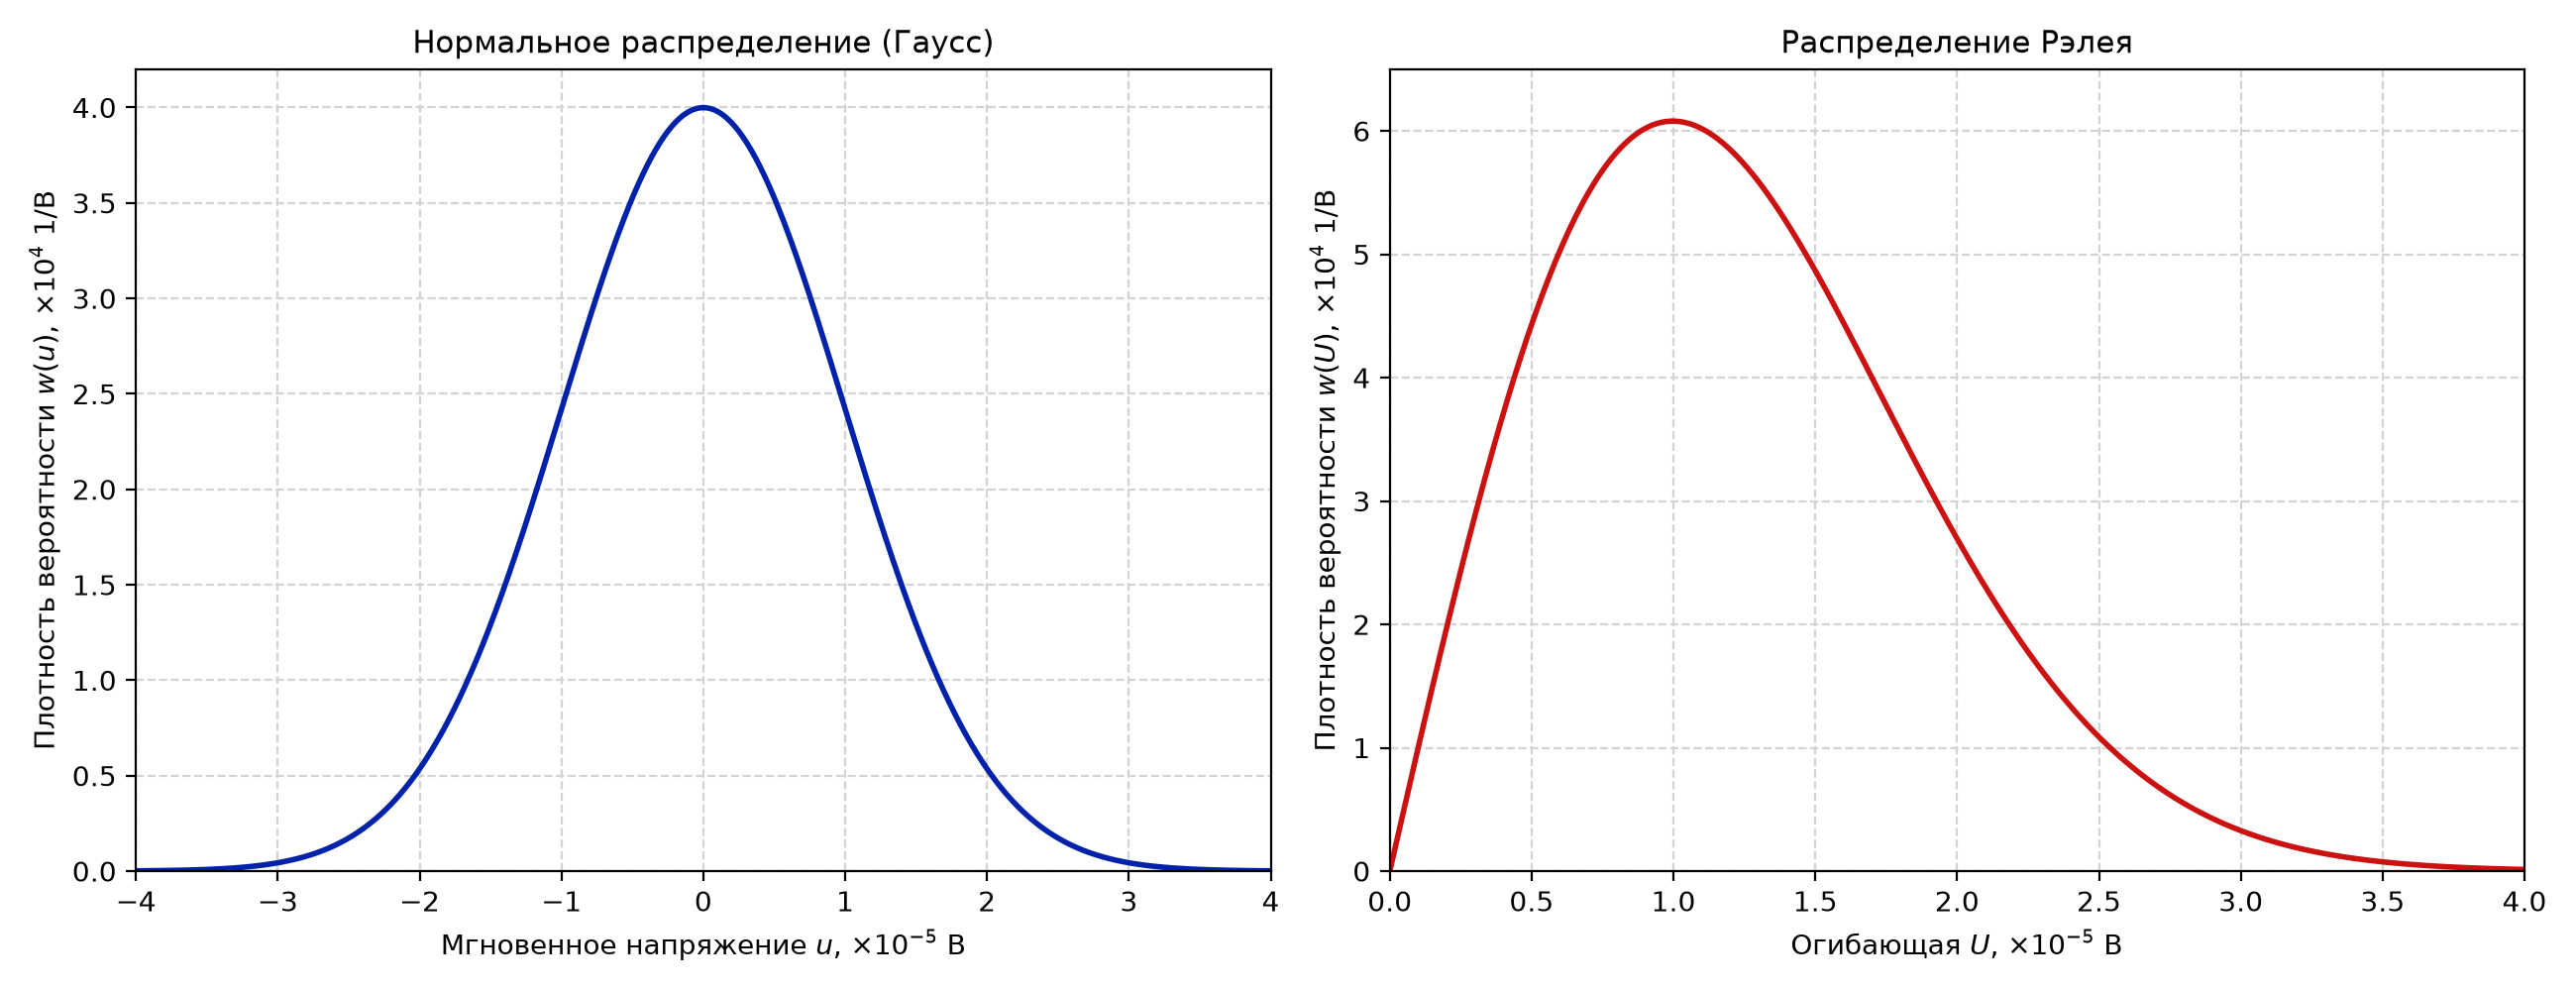
\includegraphics[width=0.88\linewidth]{exports_fig/pic_task_2_1.png}
    \caption{Плотности вероятностей мгновенных значений напряжения $w(u)$ и огибающей шума $w(U)$ на выходе преселектора}
    \label{fig:task_2_1}
\end{figure}

По графикам (Рис.~\ref{fig:task_2_1}) видно, что плотность вероятности мгновенного напряжения симметрична относительно нулевого значения, а плотность вероятности огибающей принимает строго положительные значения.

\subsection{Решение задачи №2-2}

При воздействии на входе линейного амплитудного детектора (АД) квазигармонического шума среднее значение выходного напряжения равно $\overline{U}_{\text{вых}} = 0{,}1$~В. Определить эффективное (среднеквадратическое) напряжение флуктуаций шума на выходе детектора $\sigma_u$.

\paragraph{Решение.}
Поскольку полезный сигнал на входе отсутствует ($a = U_c / U_{\text{ш}} = 0$), огибающая входного узкополосного шума подчиняется закону распределения Рэлея.

Постоянная составляющая (математическое ожидание) напряжения на выходе линейного АД с коэффициентом передачи $K_{\text{д}}$ определяется первым начальным моментом рэлеевского распределения:
\begin{equation}
    \overline{U}_{\text{вых}} = K_{\text{д}} U_{\text{ш}} \sqrt{\frac{\pi}{2}} = 0{,}1\text{ В},
\end{equation}
откуда величина масштабированного входного шума составляет:
\begin{equation}
    K_{\text{д}} U_{\text{ш}} = \frac{\overline{U}_{\text{вых}}}{\sqrt{\frac{\pi}{2}}} = \frac{0{,}1}{\sqrt{\frac{\pi}{2}}} \approx 0{,}0798\text{ В} \approx 0{,}08\text{ В}.
\end{equation}

Дисперсия огибающей на выходе линейного АД определяется центральным моментом второго порядка закона Рэлея:
\begin{equation}
    \sigma_u^2 = K_{\text{д}}^2 U_{\text{ш}}^2 \left( 2 - \frac{\pi}{2} \right) = K_{\text{д}}^2 U_{\text{ш}}^2 \frac{4 - \pi}{2}.
\end{equation}

Тогда эффективное (среднеквадратическое) напряжение случайной составляющей шума на выходе АД равно:
\begin{equation}
    \sigma_u = K_{\text{д}} U_{\text{ш}} \sqrt{\frac{4 - \pi}{2}} = 0{,}0798 \cdot \sqrt{\frac{4 - \pi}{2}} \approx 0{,}052\text{ В} \approx 52\text{ мВ}.
\end{equation}

Связь между среднеквадратическим отклонением и постоянной составляющей можно выразить непосредственно через коэффициент формы рэлеевского распределения:
\begin{equation}
    \sigma_u = \overline{U}_{\text{вых}} \sqrt{\frac{4 - \pi}{\pi}} = 0{,}1 \cdot 0{,}5227 \approx 0{,}052\text{ В}.
\end{equation}

\begin{figure}[H]
    \centering
    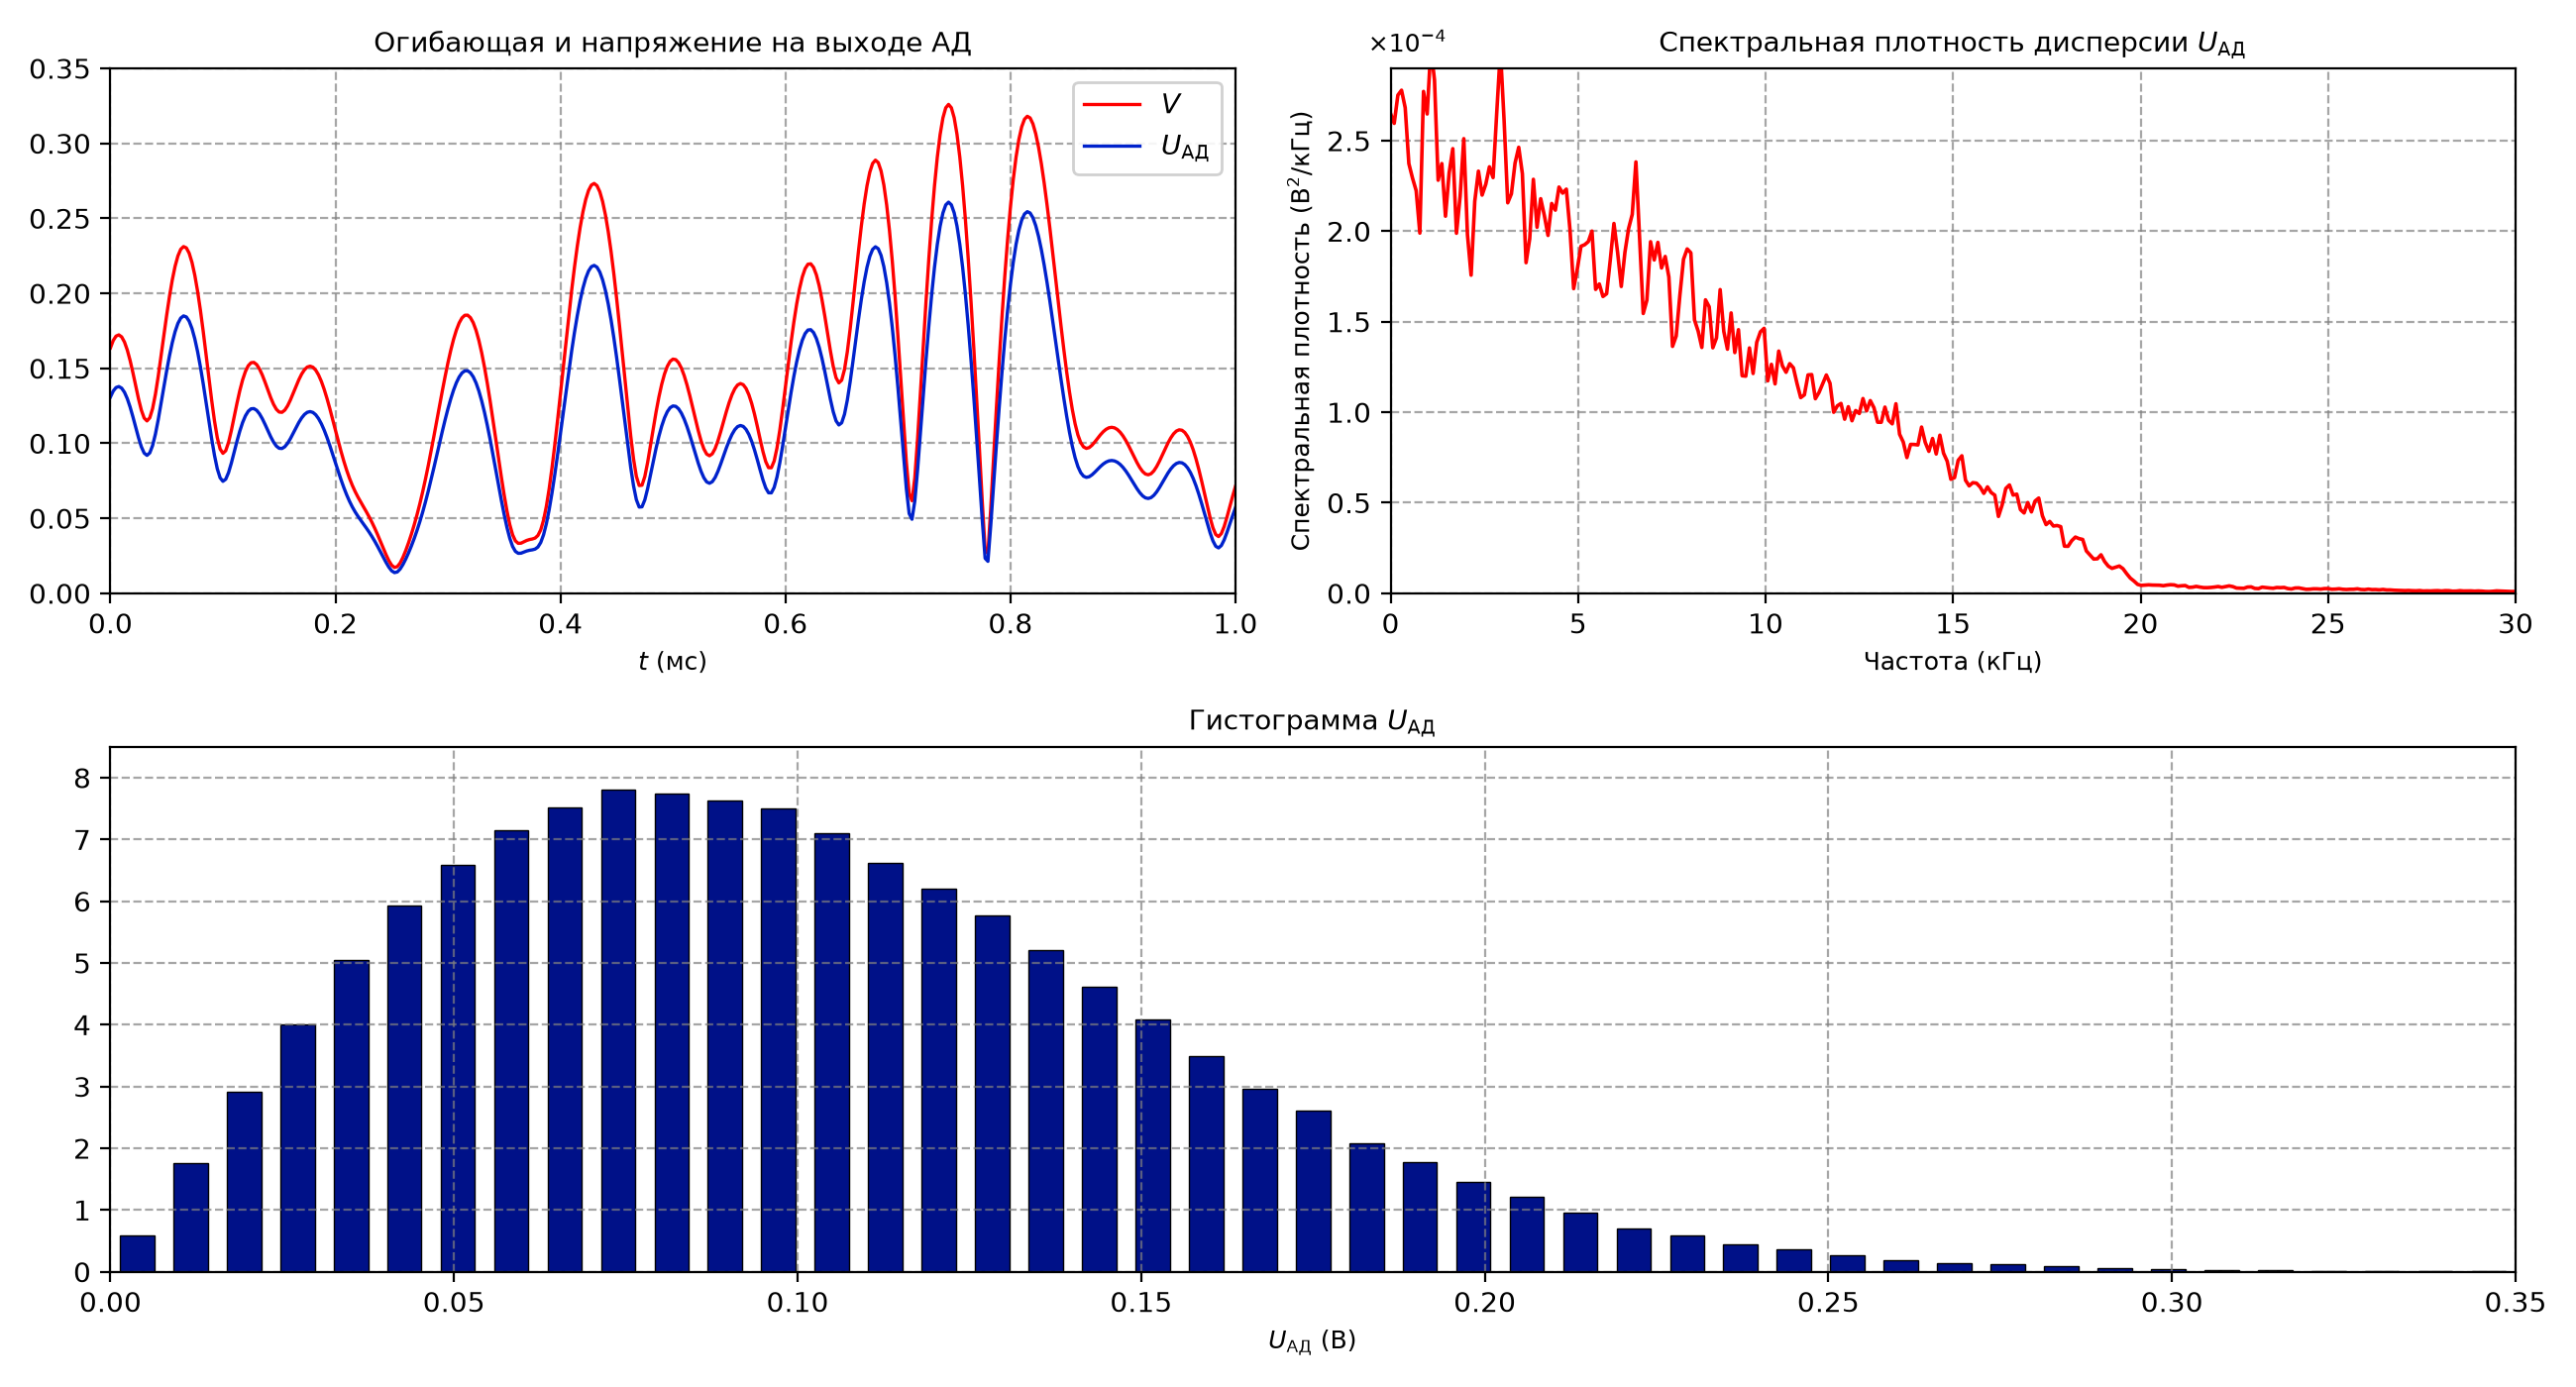
\includegraphics[width=0.92\linewidth]{exports_fig/pic_ad_kd08_results.png}
    \caption{Характеристики процессов на выходе линейного АД при воздействии квазигармонического шума ($K_{\text{д}} = 0{,}8$)}
    \label{fig:ad_kd08_results}
\end{figure}

\subsection{Решение задачи №2-3}

При действии квазигармонического шума на входе линейного амплитудного детектора с коэффициентом передачи $K_{\text{д}} = 0{,}8$ постоянная составляющая выходного напряжения составляет $\overline{U}_{\text{вых}} = 0{,}1$~В. 
Требуется:
\begin{enumerate}
    \item Рассчитать постоянную составляющую выходного напряжения $\overline{U}_{\text{д}}$, если на вход АД дополнительно подать немодулированный гармонический сигнал с амплитудой $U_c = 0{,}3$~В.
    \item Построить зависимости постоянной составляющей $\overline{U}$ и эффективного значения переменной составляющей шума $\sigma_u$ на выходе АД от амплитуды сигнала $U_c$.
\end{enumerate}

\paragraph{Решение.}
Определим эффективное напряжение узкополосного входного шума $U_{\text{ш}}$ при отсутствии сигнала ($U_c = 0$):
\begin{equation}
    \overline{U}_{\text{вых}} = K_{\text{д}} U_{\text{ш}} \sqrt{\frac{\pi}{2}} = 0{,}1\text{ В} \quad \Longrightarrow \quad U_{\text{ш}} = \frac{0{,}1}{0{,}8 \cdot \sqrt{\frac{\pi}{2}}} \approx 0{,}1\text{ В}.
\end{equation}

При подаче сигнала с амплитудой $U_c = 0{,}3$~В отношение сигнал/шум по напряжению на входе детектора равно:
\begin{equation}
    a = \frac{U_c}{U_{\text{ш}}} = \frac{0{,}3}{0{,}1} = 3.
\end{equation}

Огибающая смеси гармонического колебания и квазигармонического шума подчиняется закону распределения Райса. Постоянная составляющая на выходе линейного АД определяется выражением:
\begin{equation}
    \overline{U}_{\text{д}} = K_{\text{д}} U_{\text{ш}} M(a).
\end{equation}

Для надпороговой области ($a \ge 3$) значение коэффициента $M(a)$ с высокой точностью аппроксимируется соотношением:
\begin{equation}
    M(a) \approx \sqrt{a^2 + 1} = \sqrt{3^2 + 1} = \sqrt{10} \approx 3{,}162.
\end{equation}

Следовательно, постоянная составляющая напряжения на выходе детектора составляет:
\begin{equation}
    \overline{U}_{\text{д}} = 0{,}8 \cdot 0{,}1 \cdot 3{,}162 \approx 0{,}254\text{ В}.
\end{equation}

\paragraph{Анализ зависимостей от амплитуды сигнала.}
Результаты имитационного моделирования в диапазоне амплитуд входного сигнала $U_c \in [0; 1{,}0]$~В сведены в Таблицу~\ref{tab:task_2_3_data} и сопоставлены с теоретическими кривыми на Рис.~\ref{fig:task_2_3_curves}.

\begin{table}[H]
\centering
\small
\setlength{\tabcolsep}{3.2pt}
\caption{Статистические характеристики напряжения на выходе АД при вариации амплитуды сигнала}
\label{tab:task_2_3_data}
\begin{tabular}{|l|c|c|c|c|c|c|c|c|c|c|c|c|}
\hline
$U_c$, В & 0 & 0{,}05 & 0{,}1 & 0{,}2 & 0{,}3 & 0{,}4 & 0{,}5 & 0{,}6 & 0{,}7 & 0{,}8 & 0{,}9 & 1{,}0 \\ \hline
$\overline{U}$, В & 0{,}100 & 0{,}106 & 0{,}124 & 0{,}182 & 0{,}254 & 0{,}330 & 0{,}408 & 0{,}487 & 0{,}565 & 0{,}645 & 0{,}725 & 0{,}804 \\ \hline
$\sigma_u$, В & 0{,}052 & 0{,}055 & 0{,}062 & 0{,}073 & 0{,}077 & 0{,}079 & 0{,}079 & 0{,}079 & 0{,}080 & 0{,}080 & 0{,}080 & 0{,}080 \\ \hline
\end{tabular}
\end{table}

\begin{figure}[H]
    \centering
    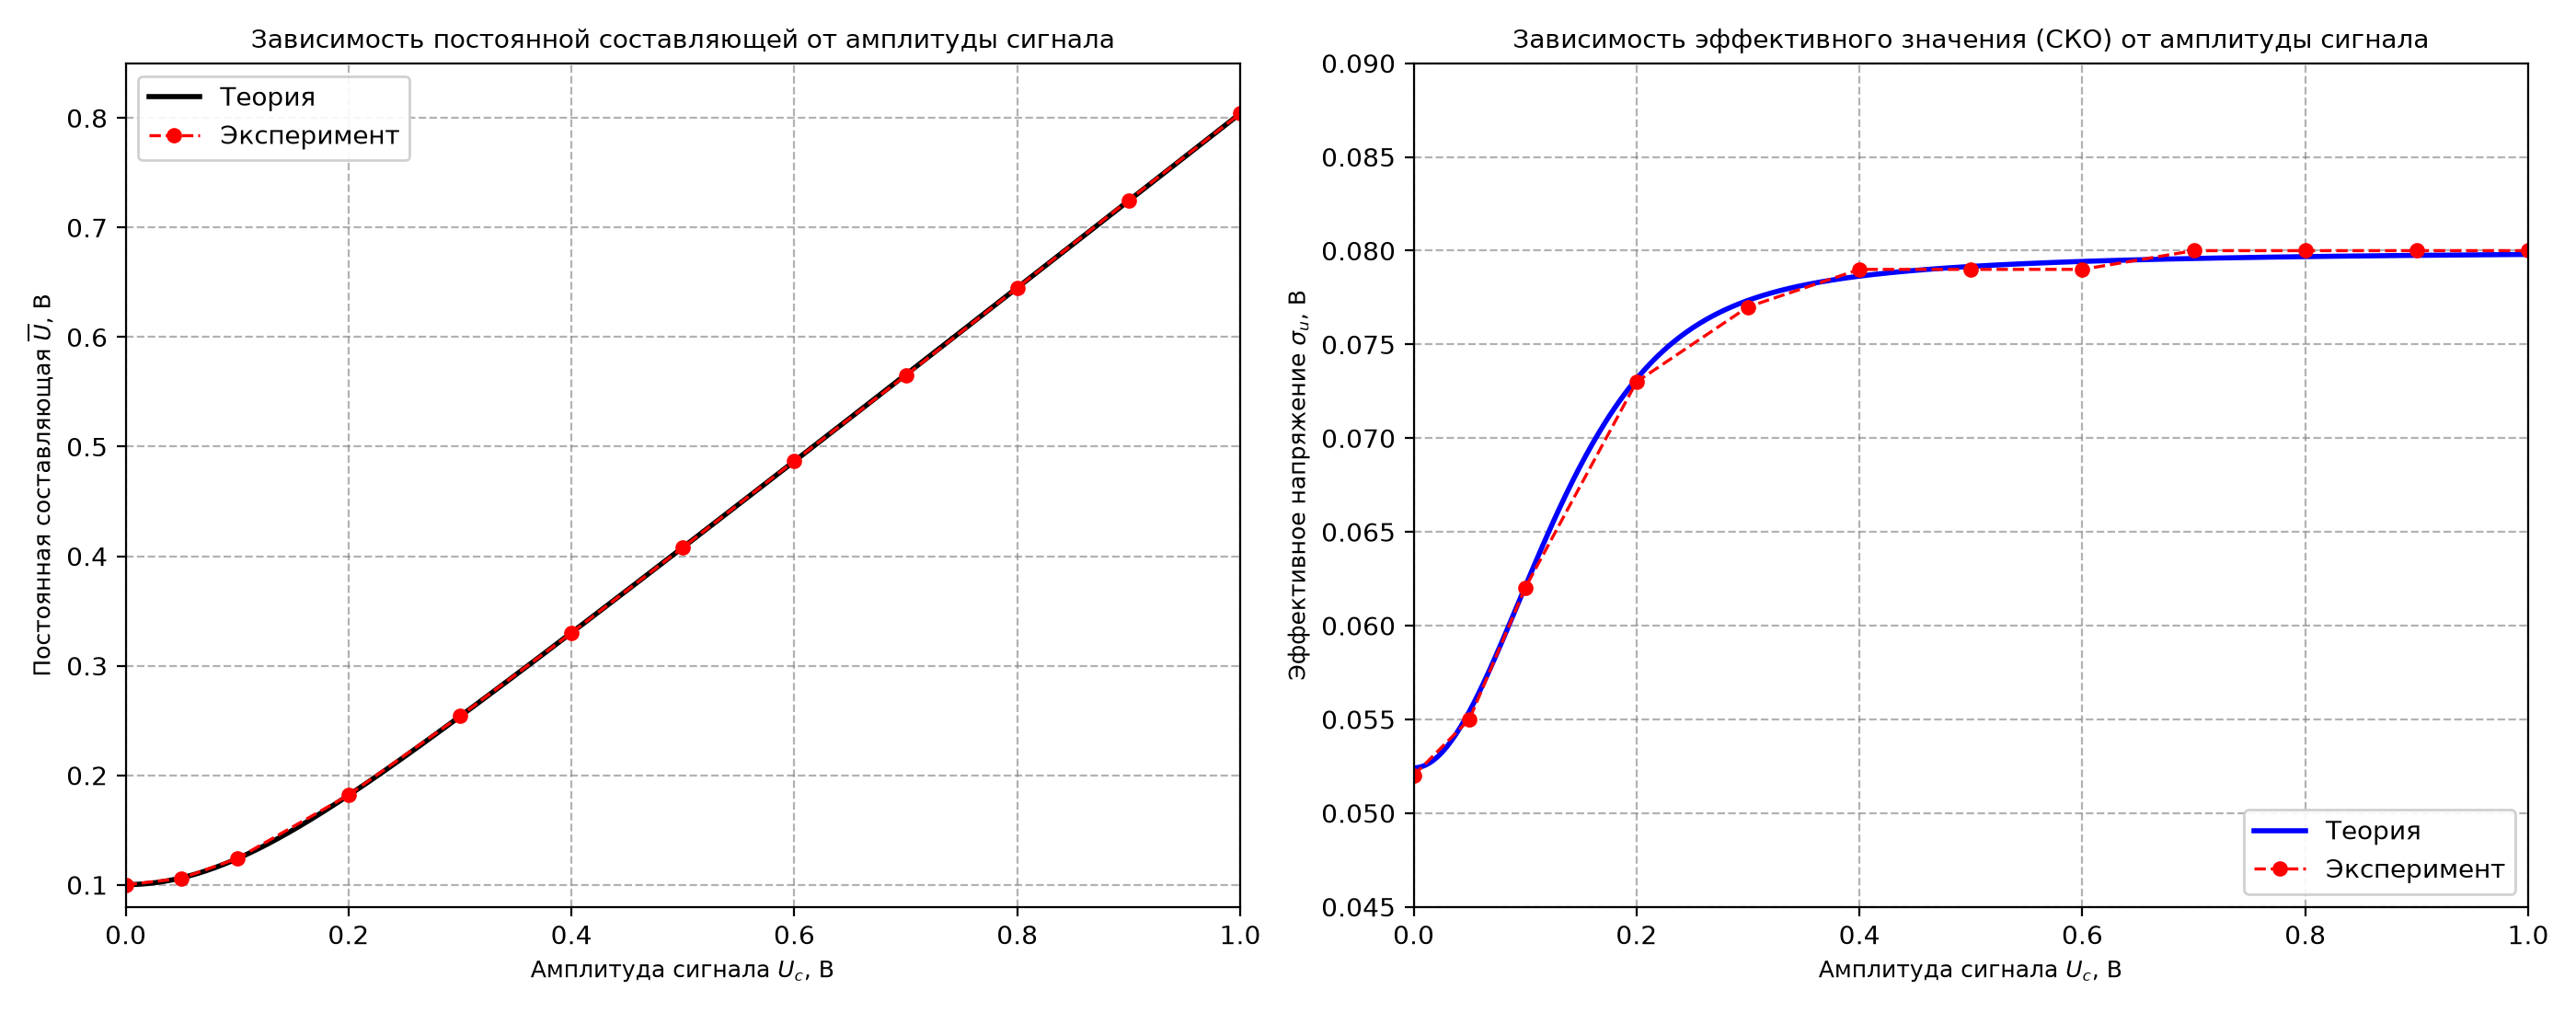
\includegraphics[width=0.95\linewidth]{exports_fig/pic_task_2_3_curves.png}
    \caption{Теоретические и экспериментальные зависимости постоянной составляющей $\overline{U}$ и эффективного напряжения шума $\sigma_u$ на выходе АД от амплитуды сигнала $U_c$}
    \label{fig:task_2_3_curves}
\end{figure}

 При слабом сигнале ($U_c < 0{,}1$~В, $a < 1$) постоянная составляющая изменяется медленно по параболическому закону, что иллюстрирует эффект подавления слабого сигнала сильным шумом. При сильном сигнале ($a \ge 3$) зависимость становится строго линейной с крутизной, равной коэффициенту передачи детектора: $\overline{U} \approx K_{\text{д}} U_c = 0{,}8 U_c$.
 Эффективное значение переменной составляющей шума (СКО) плавно возрастает от значения рэлеевского шума $\sigma_u = K_{\text{д}} U_{\text{ш}} \sqrt{\frac{4-\pi}{2}} \approx 0{,}052$~В и асимптотически стремится к постоянному уровню $\sigma_u = K_{\text{д}} U_{\text{ш}} = 0{,}080$~В, так как синусный квадратурный шум подавляется мощной несущей, а флуктуации определяются лишь косинусной квадратурой.

 \begin{figure}[H]
    \centering
    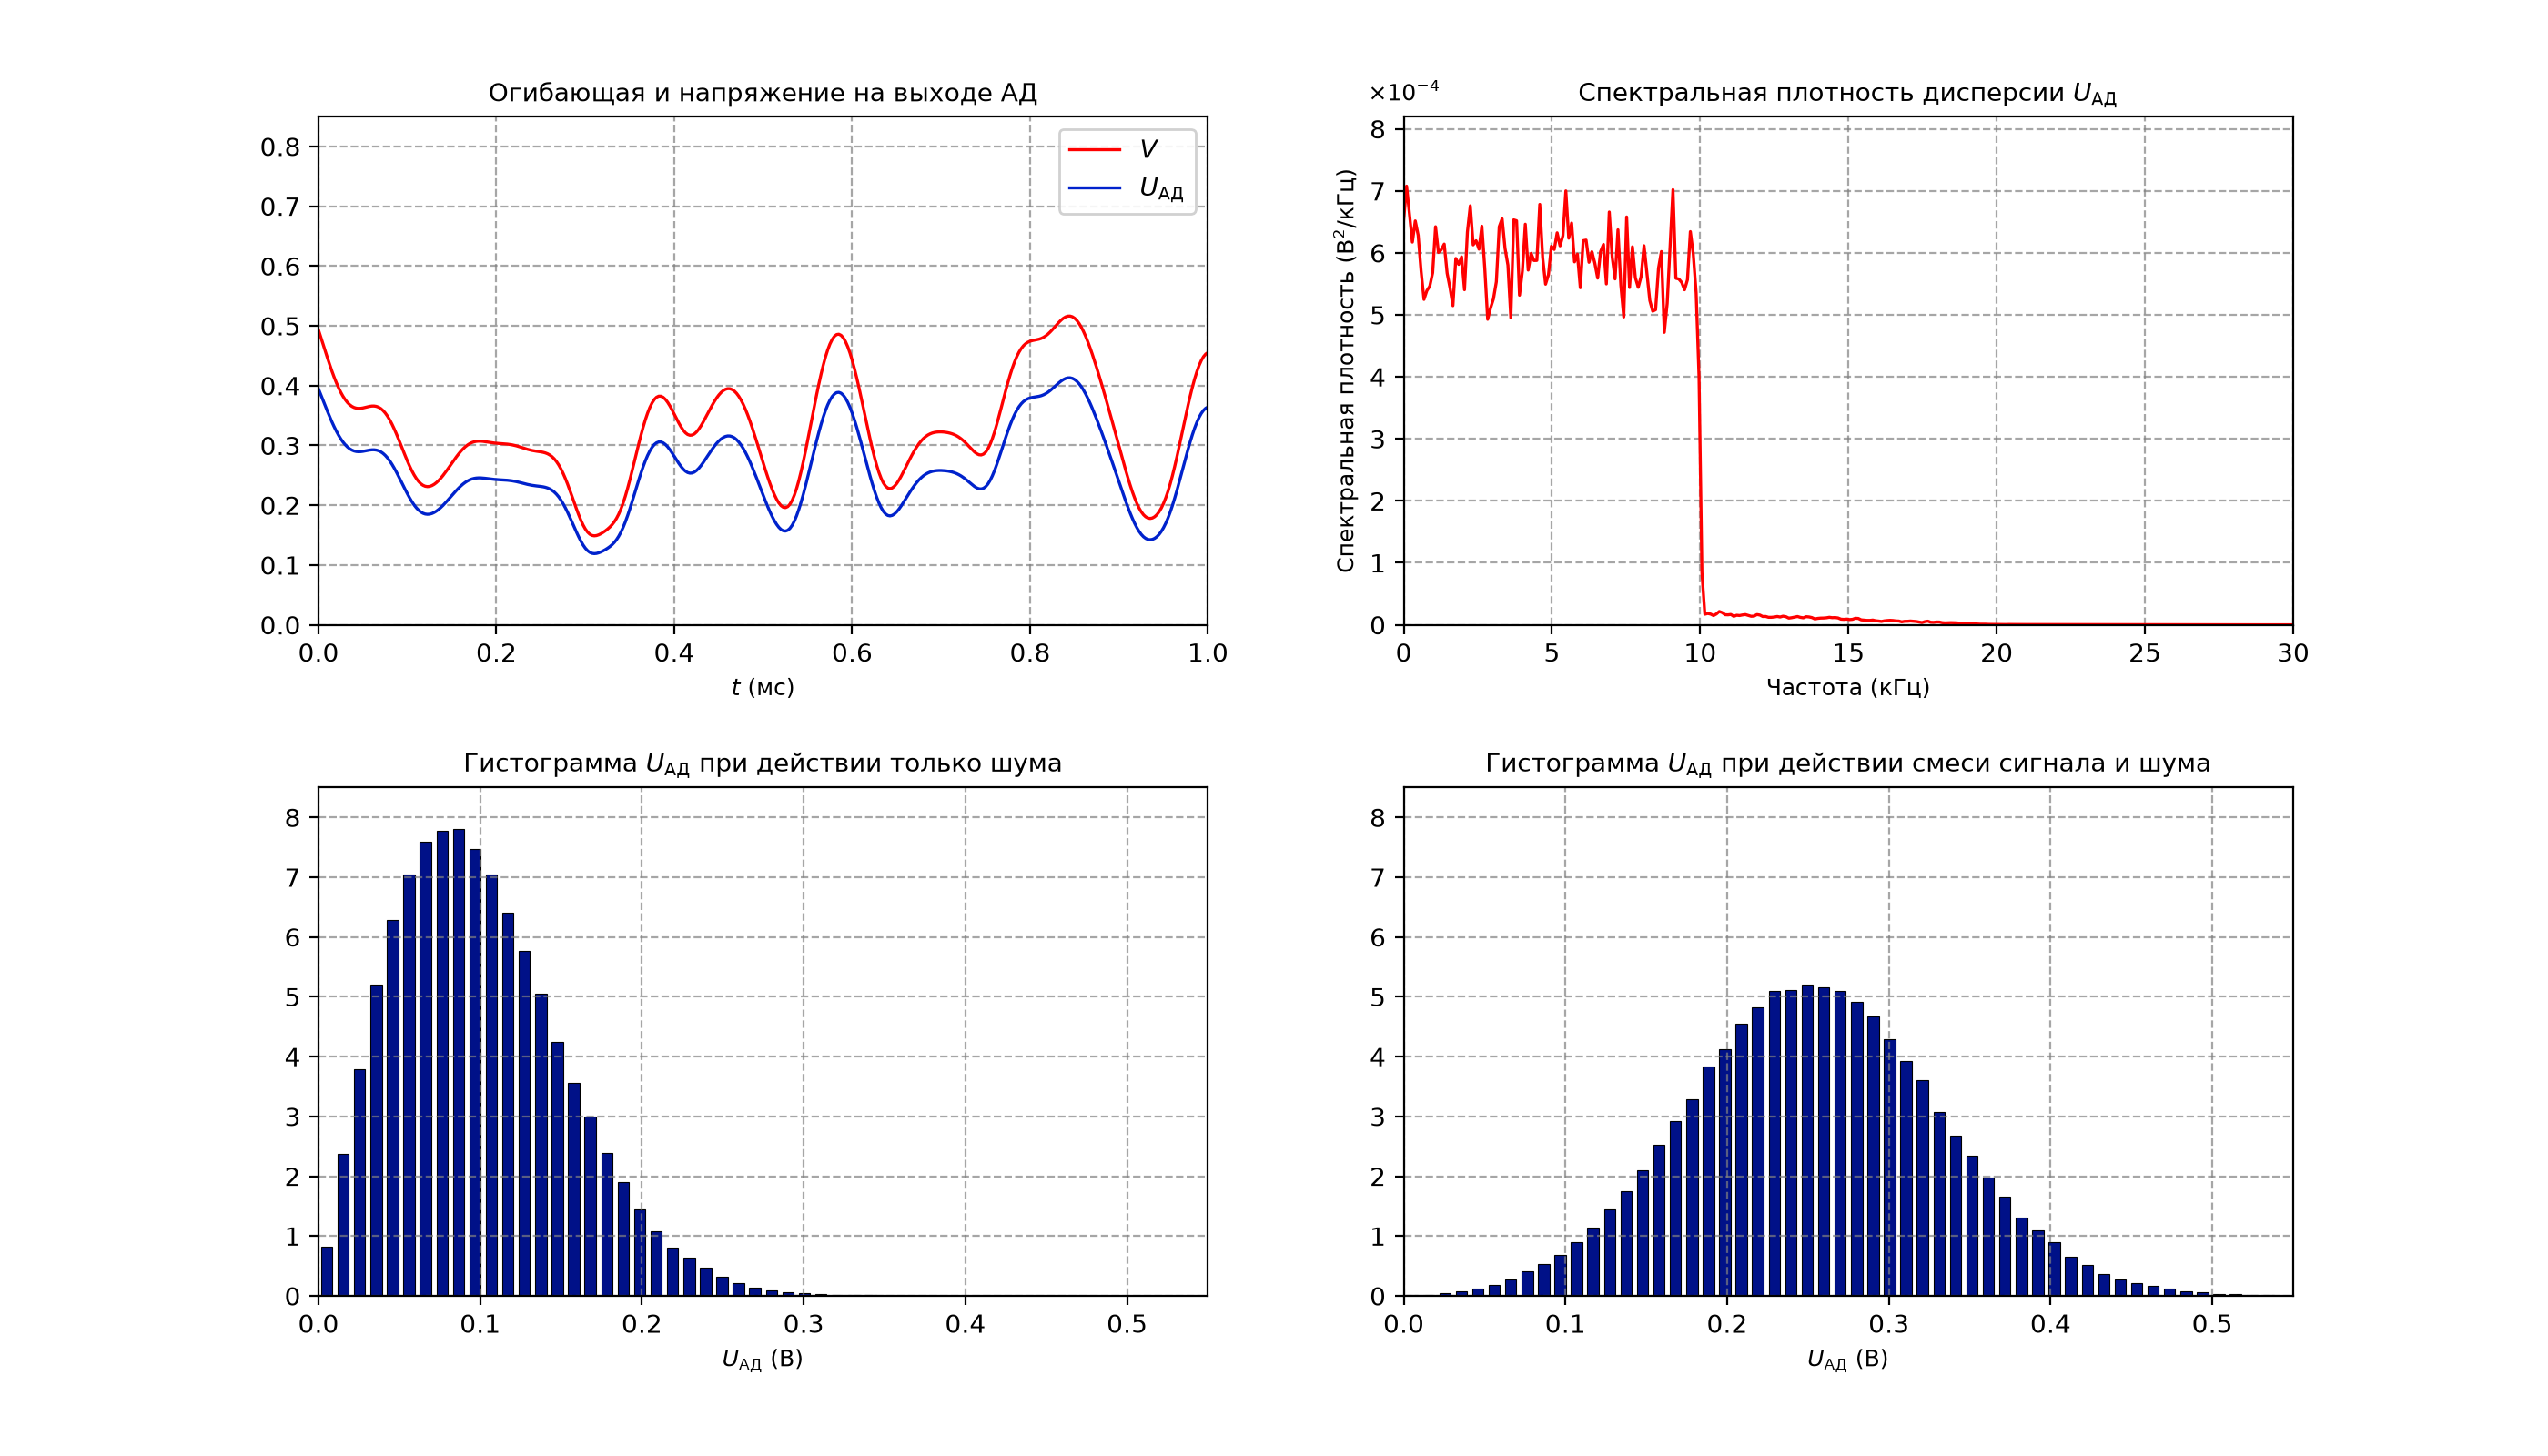
\includegraphics[width=0.95\linewidth]{exports_fig/pic_ad_uc03_results.png}
    \caption{Результаты моделирования линейного АД при подаче смеси сигнала и шума ($U_c = 0{,}3$~В, $U_{\text{ш}} = 0{,}1$~В, $K_{\text{д}} = 0{,}8$)}
    \label{fig:ad_uc03_results}
\end{figure}

Сопоставление полученных эпюр и статистических оценок (Рис.~\ref{fig:ad_uc03_results}) подтверждает, что подача сигнала с амплитудой $U_c = 0{,}3$~В смещает постоянную составляющую напряжения на выходе АД с $0{,}100$~В до $0{,}254$~В, что точно совпадает с расчётом по закону Райса при $a = 3$. Гистограмма распределения трансформируется из асимметричной рэлеевской в квазинормальную из-за подавления квадратурного синусного шума мощным вектором сигнала. При этом в спектре флуктуаций формируется прямоугольная площадка в полосе до $10$~кГц, вызванная биениями сигнала с косинусной составляющей шума
\subsection{Решение задачи №2-4}

Вольтметр измеряет постоянную составляющую напряжения на выходе линейного АД, подключённого к выходу БВЧ с шумовой полосой $\Pi_{\text{ш}} = 1$~МГц. Ко входу БВЧ подключён согласованный генератор сигналов, находящийся при стандартной температуре $T_0 = 293$~К ($+20\,^{\circ}\text{C}$). При отсутствии сигнала показания вольтметра составляют $\overline{U}_{\text{д.ш}} = 0{,}2$~В; при подаче сигнала мощностью $P_c = 5{,}07 \cdot 10^{-13}$~Вт показания увеличиваются до $\overline{U}_{\text{д.см}} = 0{,}8$~В.
Требуется определить коэффициент шума БВЧ $K_{\text{ш}}$.

\paragraph{Решение.}
Постоянная составляющая напряжения на выходе линейного АД при воздействии квазигармонического шума определяется выражением:
\begin{equation}
    \overline{U}_{\text{д.ш}} = K_{\text{д}} U_{\text{ш.вых}} \sqrt{\frac{\pi}{2}} = 0{,}2\text{ В}.
\end{equation}

При подаче смеси гармонического колебания и шума постоянная составляющая возрастает за счёт обобщённого закона Рэлея (закона Райса):
\begin{equation}
    \overline{U}_{\text{д.см}} = K_{\text{д}} U_{\text{ш.вых}} M(a) = 0{,}8\text{ В}.
\end{equation}

Разделив второе выражение на первое, найдём коэффициент функции Райса $M(a)$:
\begin{equation}
    M(a) = \frac{\overline{U}_{\text{д.см}}}{\overline{U}_{\text{д.ш}}} \sqrt{\frac{\pi}{2}} = \frac{0{,}8}{0{,}2} \sqrt{\frac{\pi}{2}} \approx 4 \cdot 1{,}2533 \approx 5{,}013.
\end{equation}

Поскольку полученное значение $M(a) > 3$, детектор работает в надпороговой области ($a \ge 3$), где применима асимптотическая зависимость $M(a) \approx \sqrt{a^2 + 1} \approx a \approx 5{,}013$.

Связь между мощностью полезного сигнала $P_c$ и суммарной мощностью шума $P_{\text{ш}}$ на входе тракта задаётся через отношение сигнал/шум по мощности $q = a^2 / 2$:
\begin{equation}
    P_{\text{ш}} = \frac{2 P_c}{a^2} = \frac{2 \cdot 5{,}07 \cdot 10^{-13}}{5{,}013^2} \approx 4{,}035 \cdot 10^{-14}\text{ Вт}.
\end{equation}

Полная мощность шума складывается из теплового шума согласованного источника $P_{\text{ш.ист}} = k T_0 \Pi_{\text{ш}}$ и приведённой ко входу мощности собственных шумов БВЧ $P_{\text{ш.соб}}'$:
\begin{equation}
    P_{\text{ш.соб}}' = P_{\text{ш}} - k T_0 \Pi_{\text{ш}} = 4{,}035 \cdot 10^{-14} - 1{,}38 \cdot 10^{-23} \cdot 293 \cdot 10^6 \approx 3{,}631 \cdot 10^{-14}\text{ Вт}.
\end{equation}

Тогда коэффициент шума БВЧ равен:
\begin{equation}
    K_{\text{ш}} = 1 + \frac{P_{\text{ш.соб}}'}{k T_0 \Pi_{\text{ш}}} = 1 + \frac{3{,}631 \cdot 10^{-14}}{4{,}043 \cdot 10^{-15}} \approx 9{,}98 \approx 10{,}0 \quad (10{,}0\text{ дБ}).
\end{equation}

\subsection{Характеристики огибающей квазигармонического колебания}

В соответствии с 8-м вариантом форма энергетического спектра входного шума задана соответствующей фильтру Баттерворта с центральной частотой $f_0 = 50$~кГц и шумовой полосой $\Pi_{\text{ш}} = 20$~кГц.

При отсутствии полезного сигнала ($U_c = 0$) квазигармонический шум представляется через низкочастотные квадратурные компоненты:
\begin{equation}
    u_{\text{ш}}(t) = U_{\text{ш}}^c(t) \cos(2\pi f_0 t) - U_{\text{ш}}^s(t) \sin(2\pi f_0 t),
\end{equation}
где $U_{\text{ш}}^c(t)$ и $U_{\text{ш}}^s(t)$ — медленно меняющиеся случайные процессы, подчиняющиеся нормальному распределению с дисперсией $\sigma^2 = U_{\text{ш}}^2 = 0{,}01$~В$^2$.

\begin{figure}[H]
    \centering
    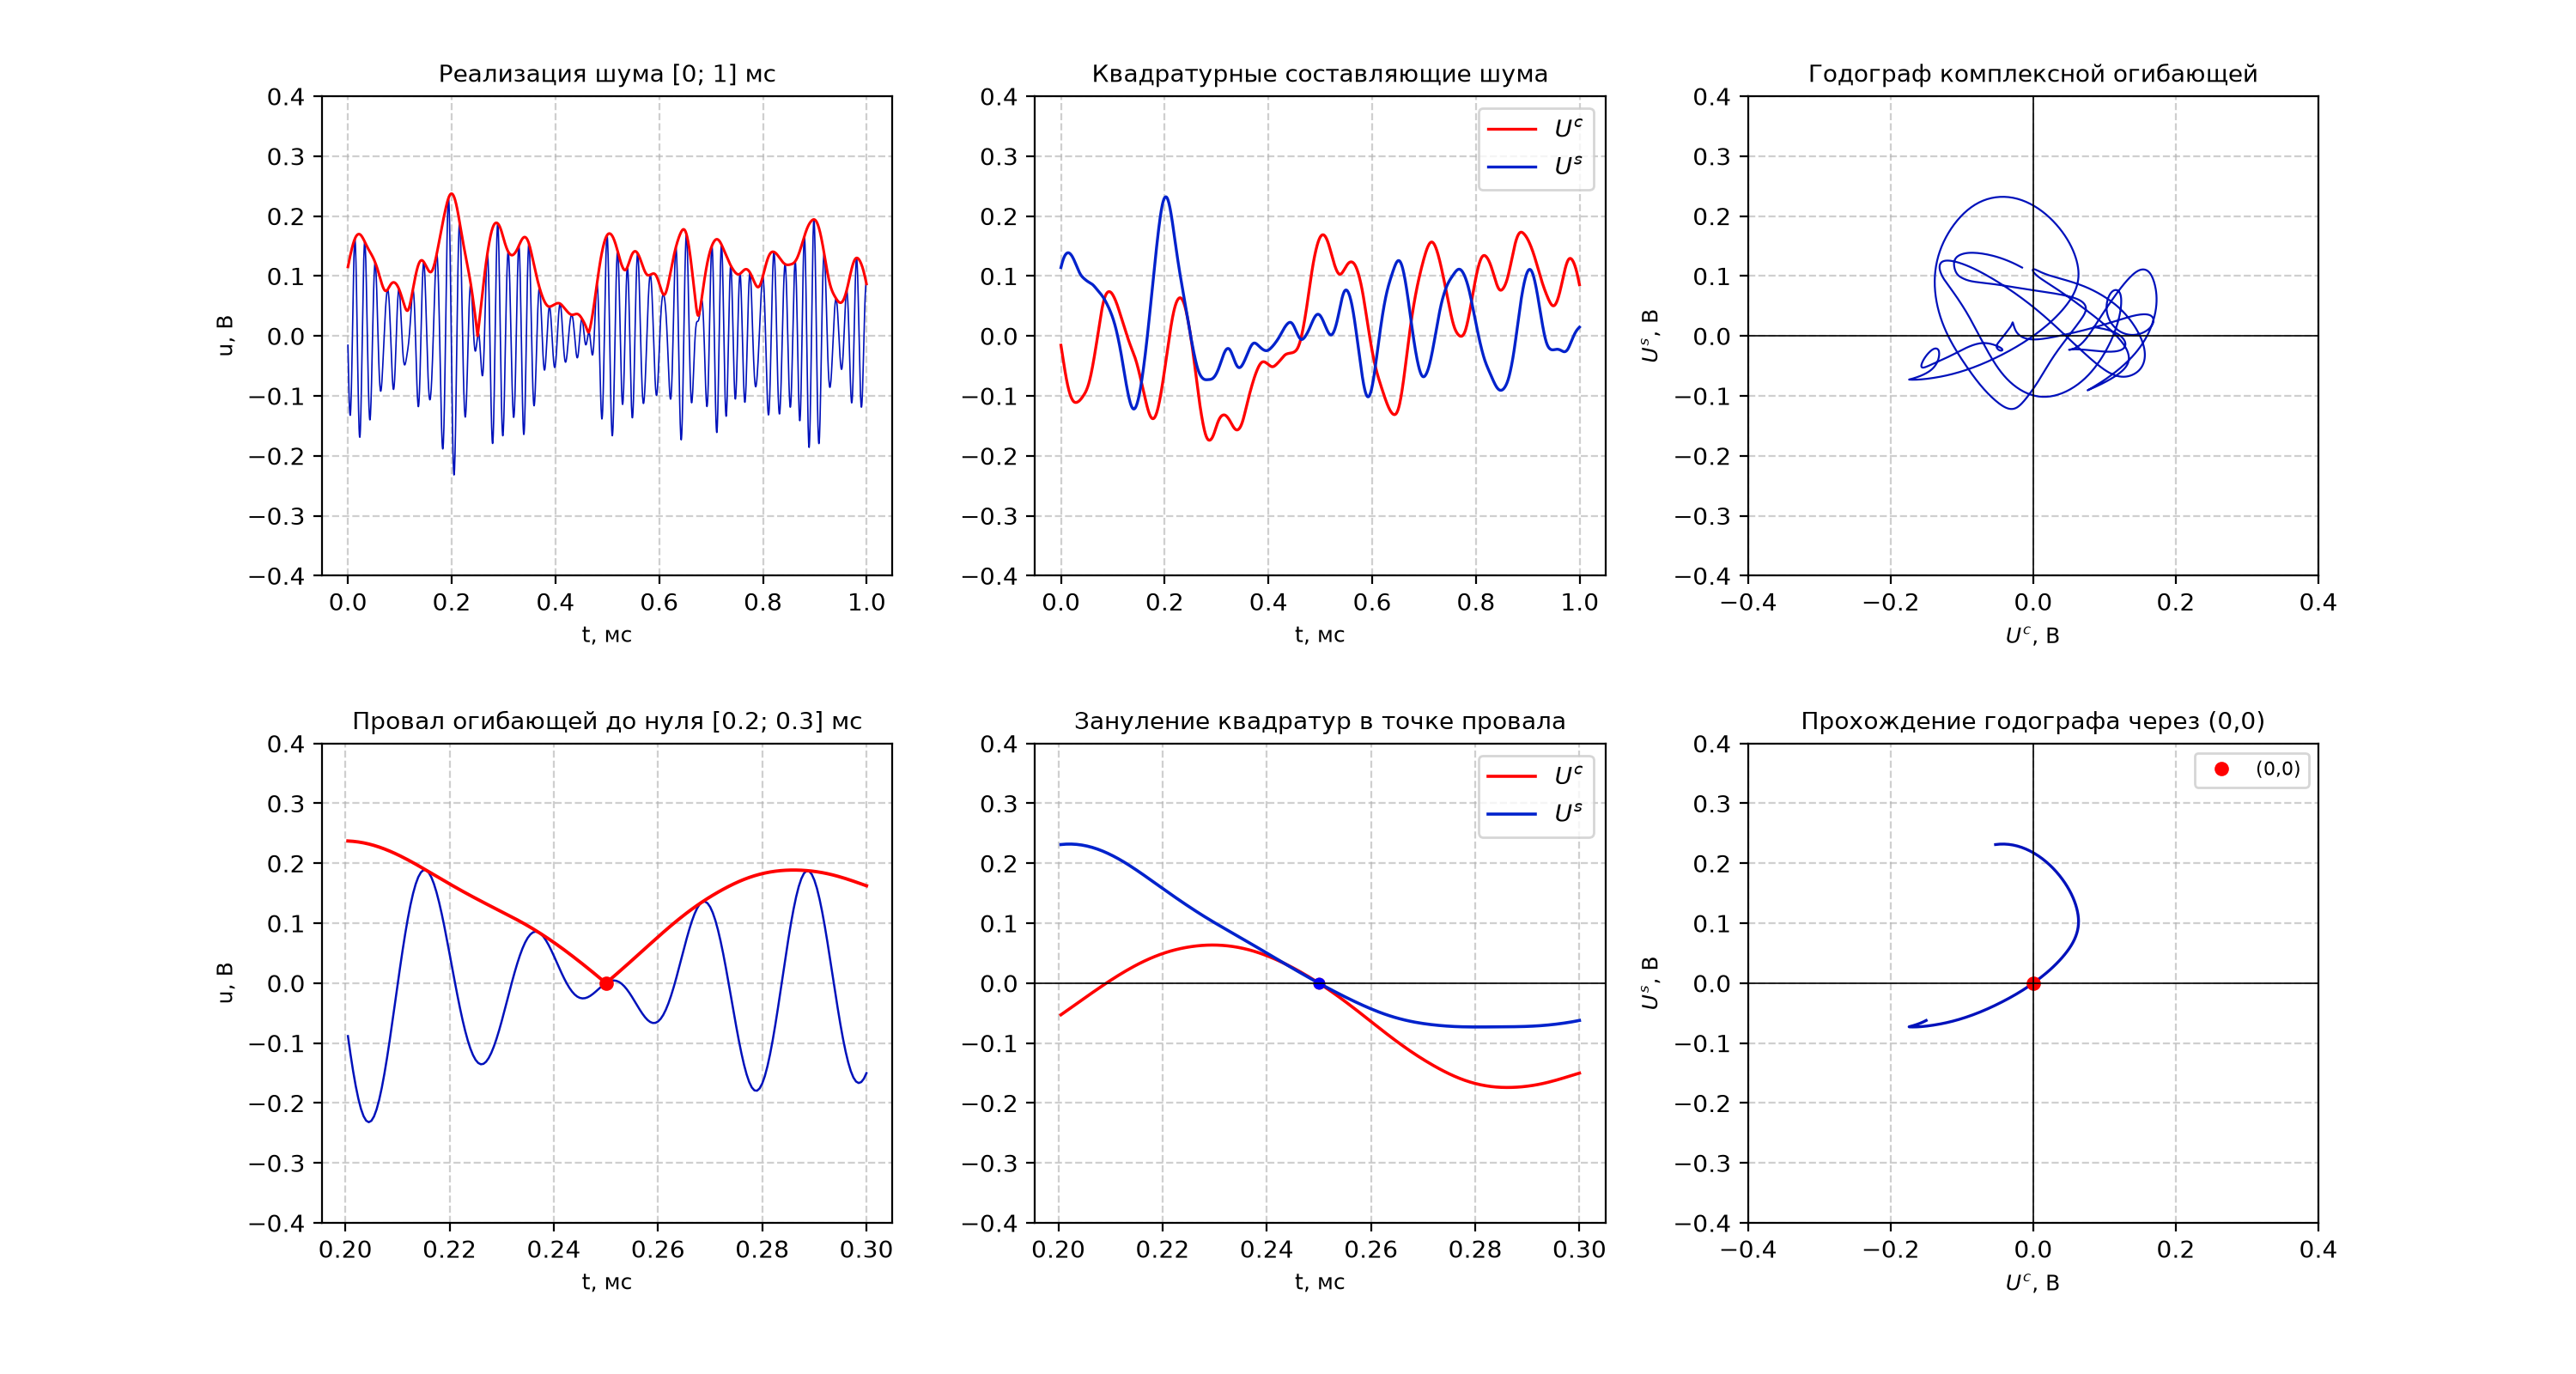
\includegraphics[width=0.96\linewidth]{exports_fig/pic_env_zero_dip.png}
    \caption{Реализации шума, квадратурные составляющие и годограф комплексной огибающей на интервале $[0; 1]$~мс и при детальном рассмотрении провала огибающей на интервале $[0{,}2; 0{,}3]$~мс}
    \label{fig:env_zero_dip}
\end{figure}

На Рис.~\ref{fig:env_zero_dip} приведена реализация шума, для которой в интервале $[0{,}2; 0{,}3]$~мс огибающая спадает практически до нуля ($V(t) \to 0$). Анализ поведения компонент показывает:
\begin{enumerate}
    \item В момент глубокого провала огибающей косинусная $U_{\text{ш}}^c(t)$ и синусная $U_{\text{ш}}^s(t)$ квадратурные составляющие одновременно обращаются в ноль.
    \item Траектория годографа комплексной огибающей $\dot{U}(t) = U_{\text{ш}}^c(t) + j U_{\text{ш}}^s(t)$ проходит непосредственно через начало координат $(0, 0)$. В этой точке фаза квазигармонического колебания претерпевает скачкообразное изменение на $\pi$, что физически приводит к резким выбросам мгновенной частоты.
\end{enumerate}

При подаче гармонического сигнала $s(t) = U_c \cos(2\pi f_0 t)$ результирующая комплексная огибающая принимает вид:
\begin{equation}
    \dot{U}_{\Sigma}(t) = \left( U_c + U_{\text{ш}}^c(t) \right) + j U_{\text{ш}}^s(t).
\end{equation}
Вектор сигнала сдвигает область блуждания годографа вправо вдоль вещественной оси на величину $U_c$.

\begin{figure}[H]
    \centering
    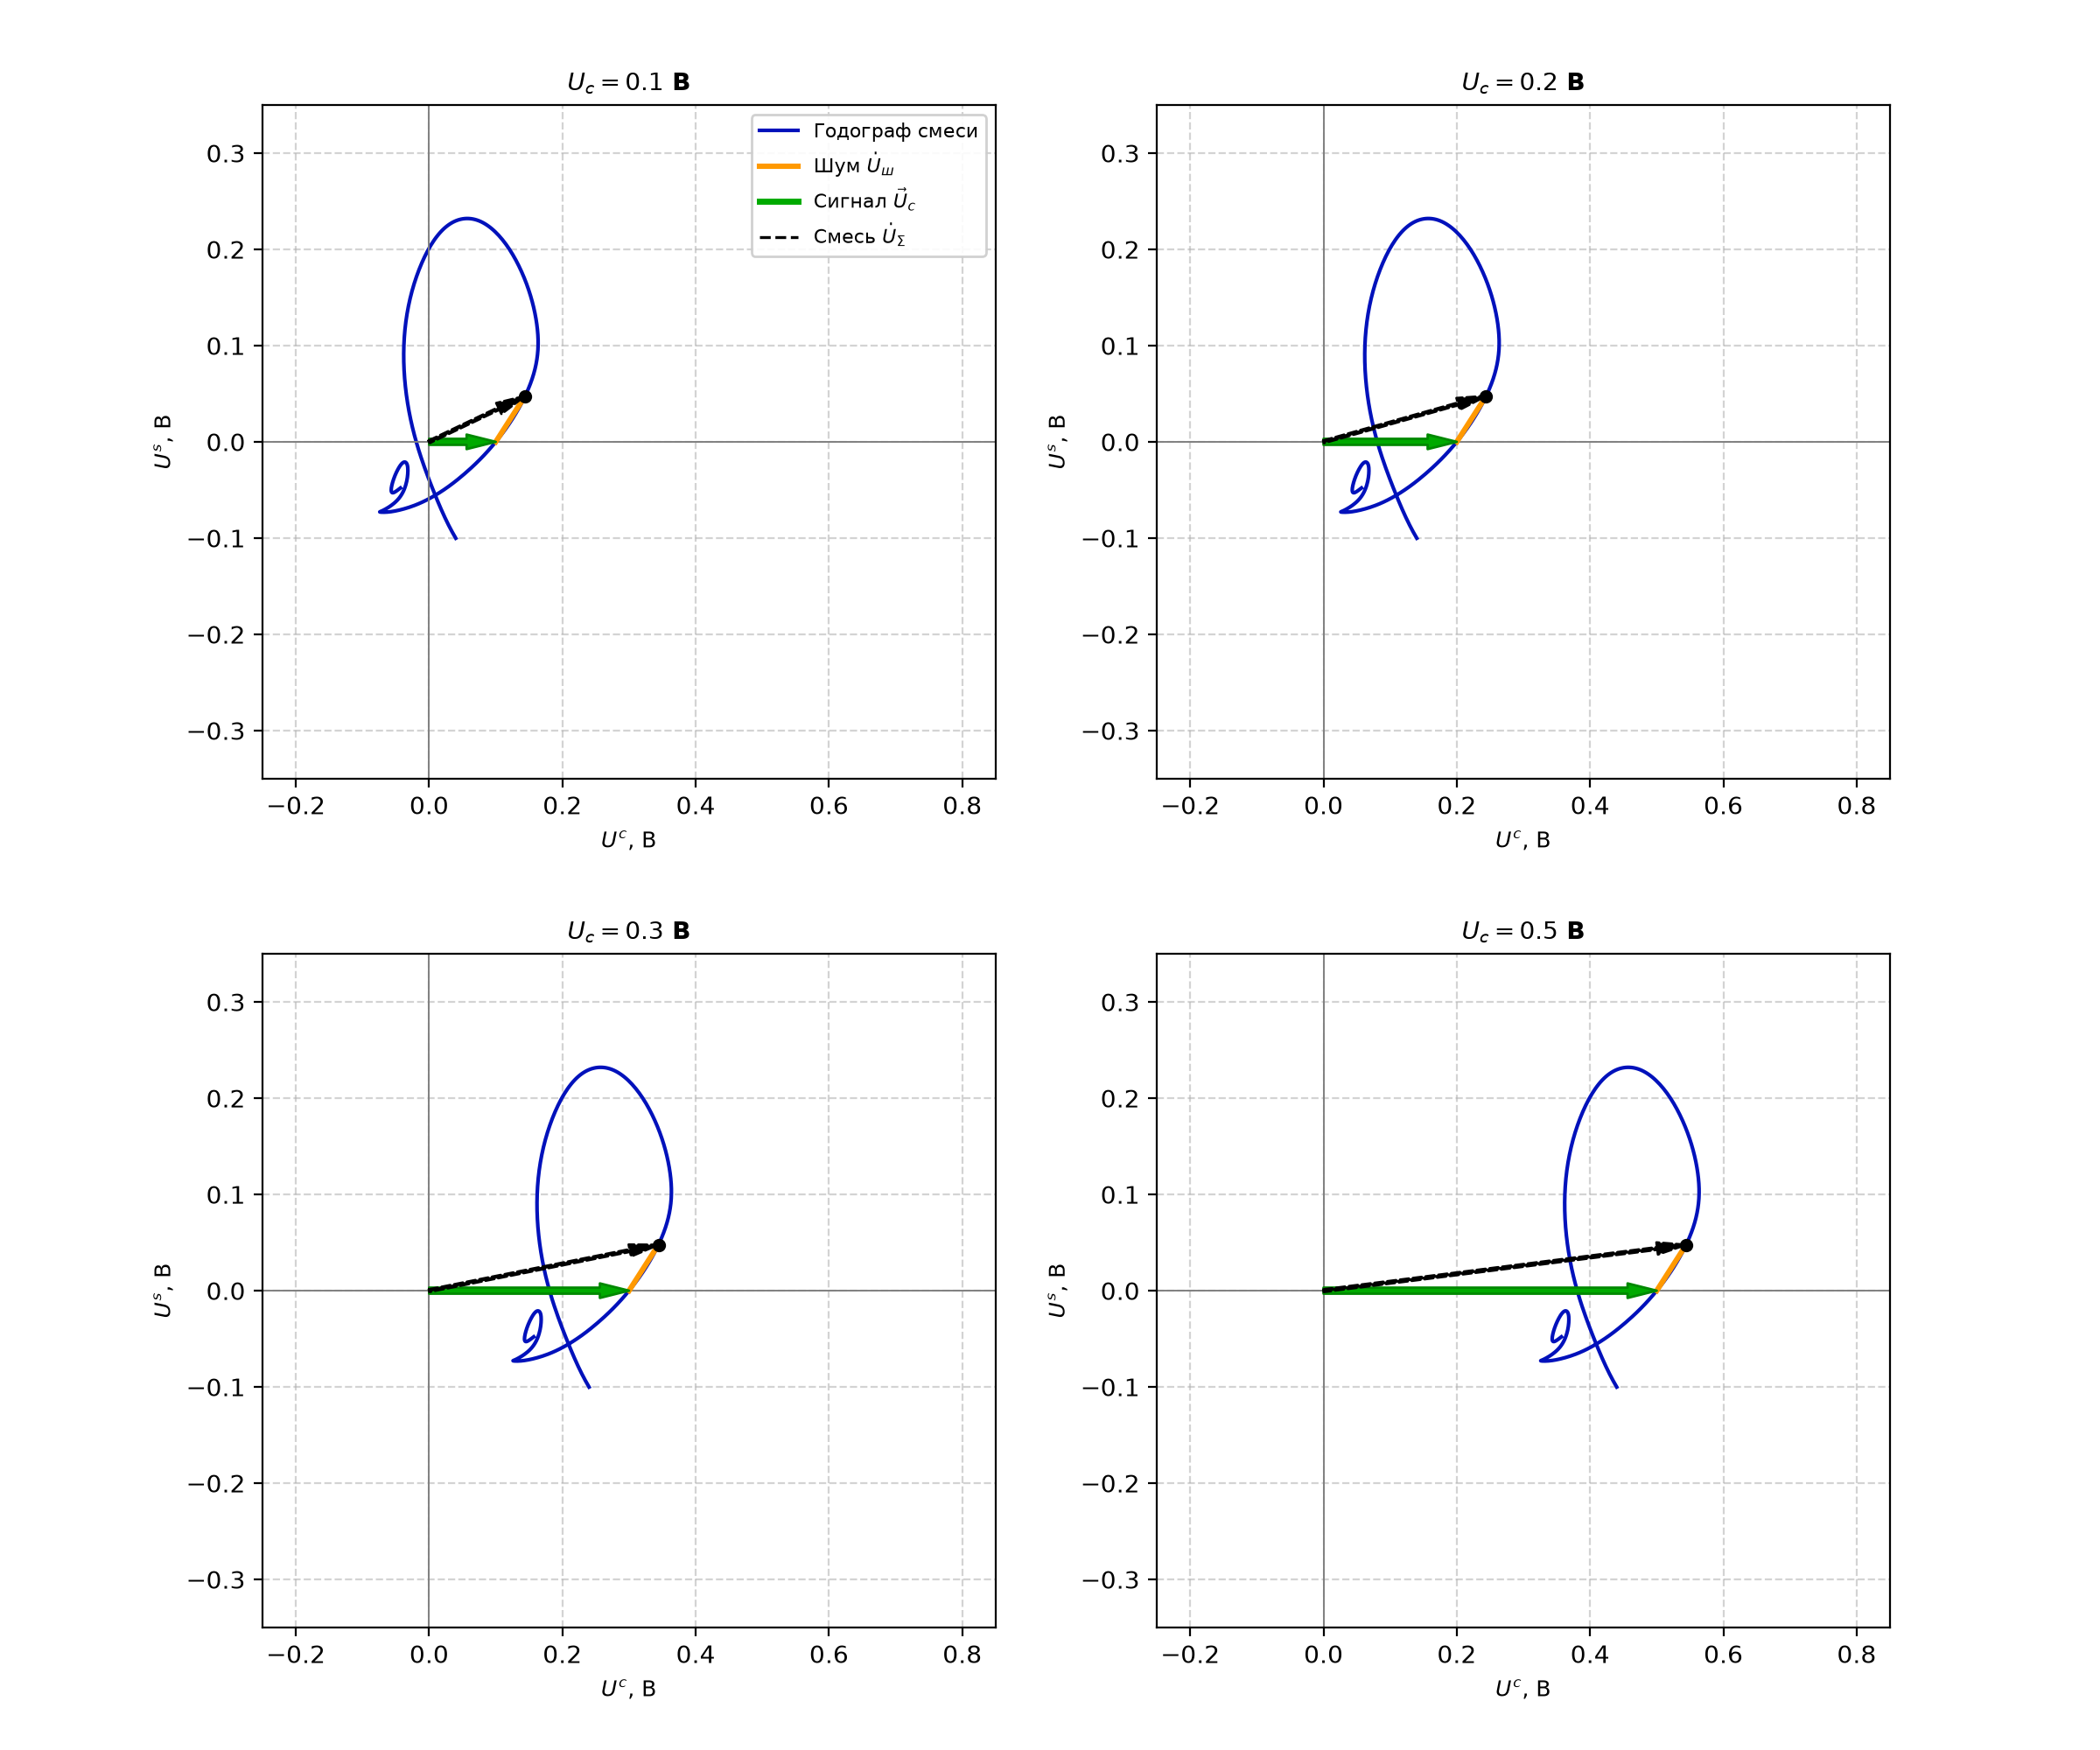
\includegraphics[width=0.88\linewidth]{exports_fig/pic_env_evolution.png}
    \caption{Эволюция годографа комплексной огибающей при увеличении амплитуды сигнала от $0{,}1$ до $0{,}5$~В}
    \label{fig:env_evolution}
\end{figure}

По графикам Рис.~\ref{fig:env_evolution} видно, что с ростом $U_c$ траектория годографа смещается в область положительных значений вещественной оси. Начиная с $U_c \ge 0{,}2$~В годограф перестаёт охватывать начало координат, фазовые флуктуации резко уменьшаются, а огибающая $V(t) \approx U_c + U_{\text{ш}}^c(t)$ практически полностью повторяет форму косинусной квадратуры шума.

Для исследования статистических свойств задана прямоугольная форма энергетического спектра шума в полосе $\Pi_{\text{ш}} = 20$~кГц при эффективном напряжении $U_{\text{ш}} = 0{,}1$~В.

\begin{figure}[H]
    \centering
    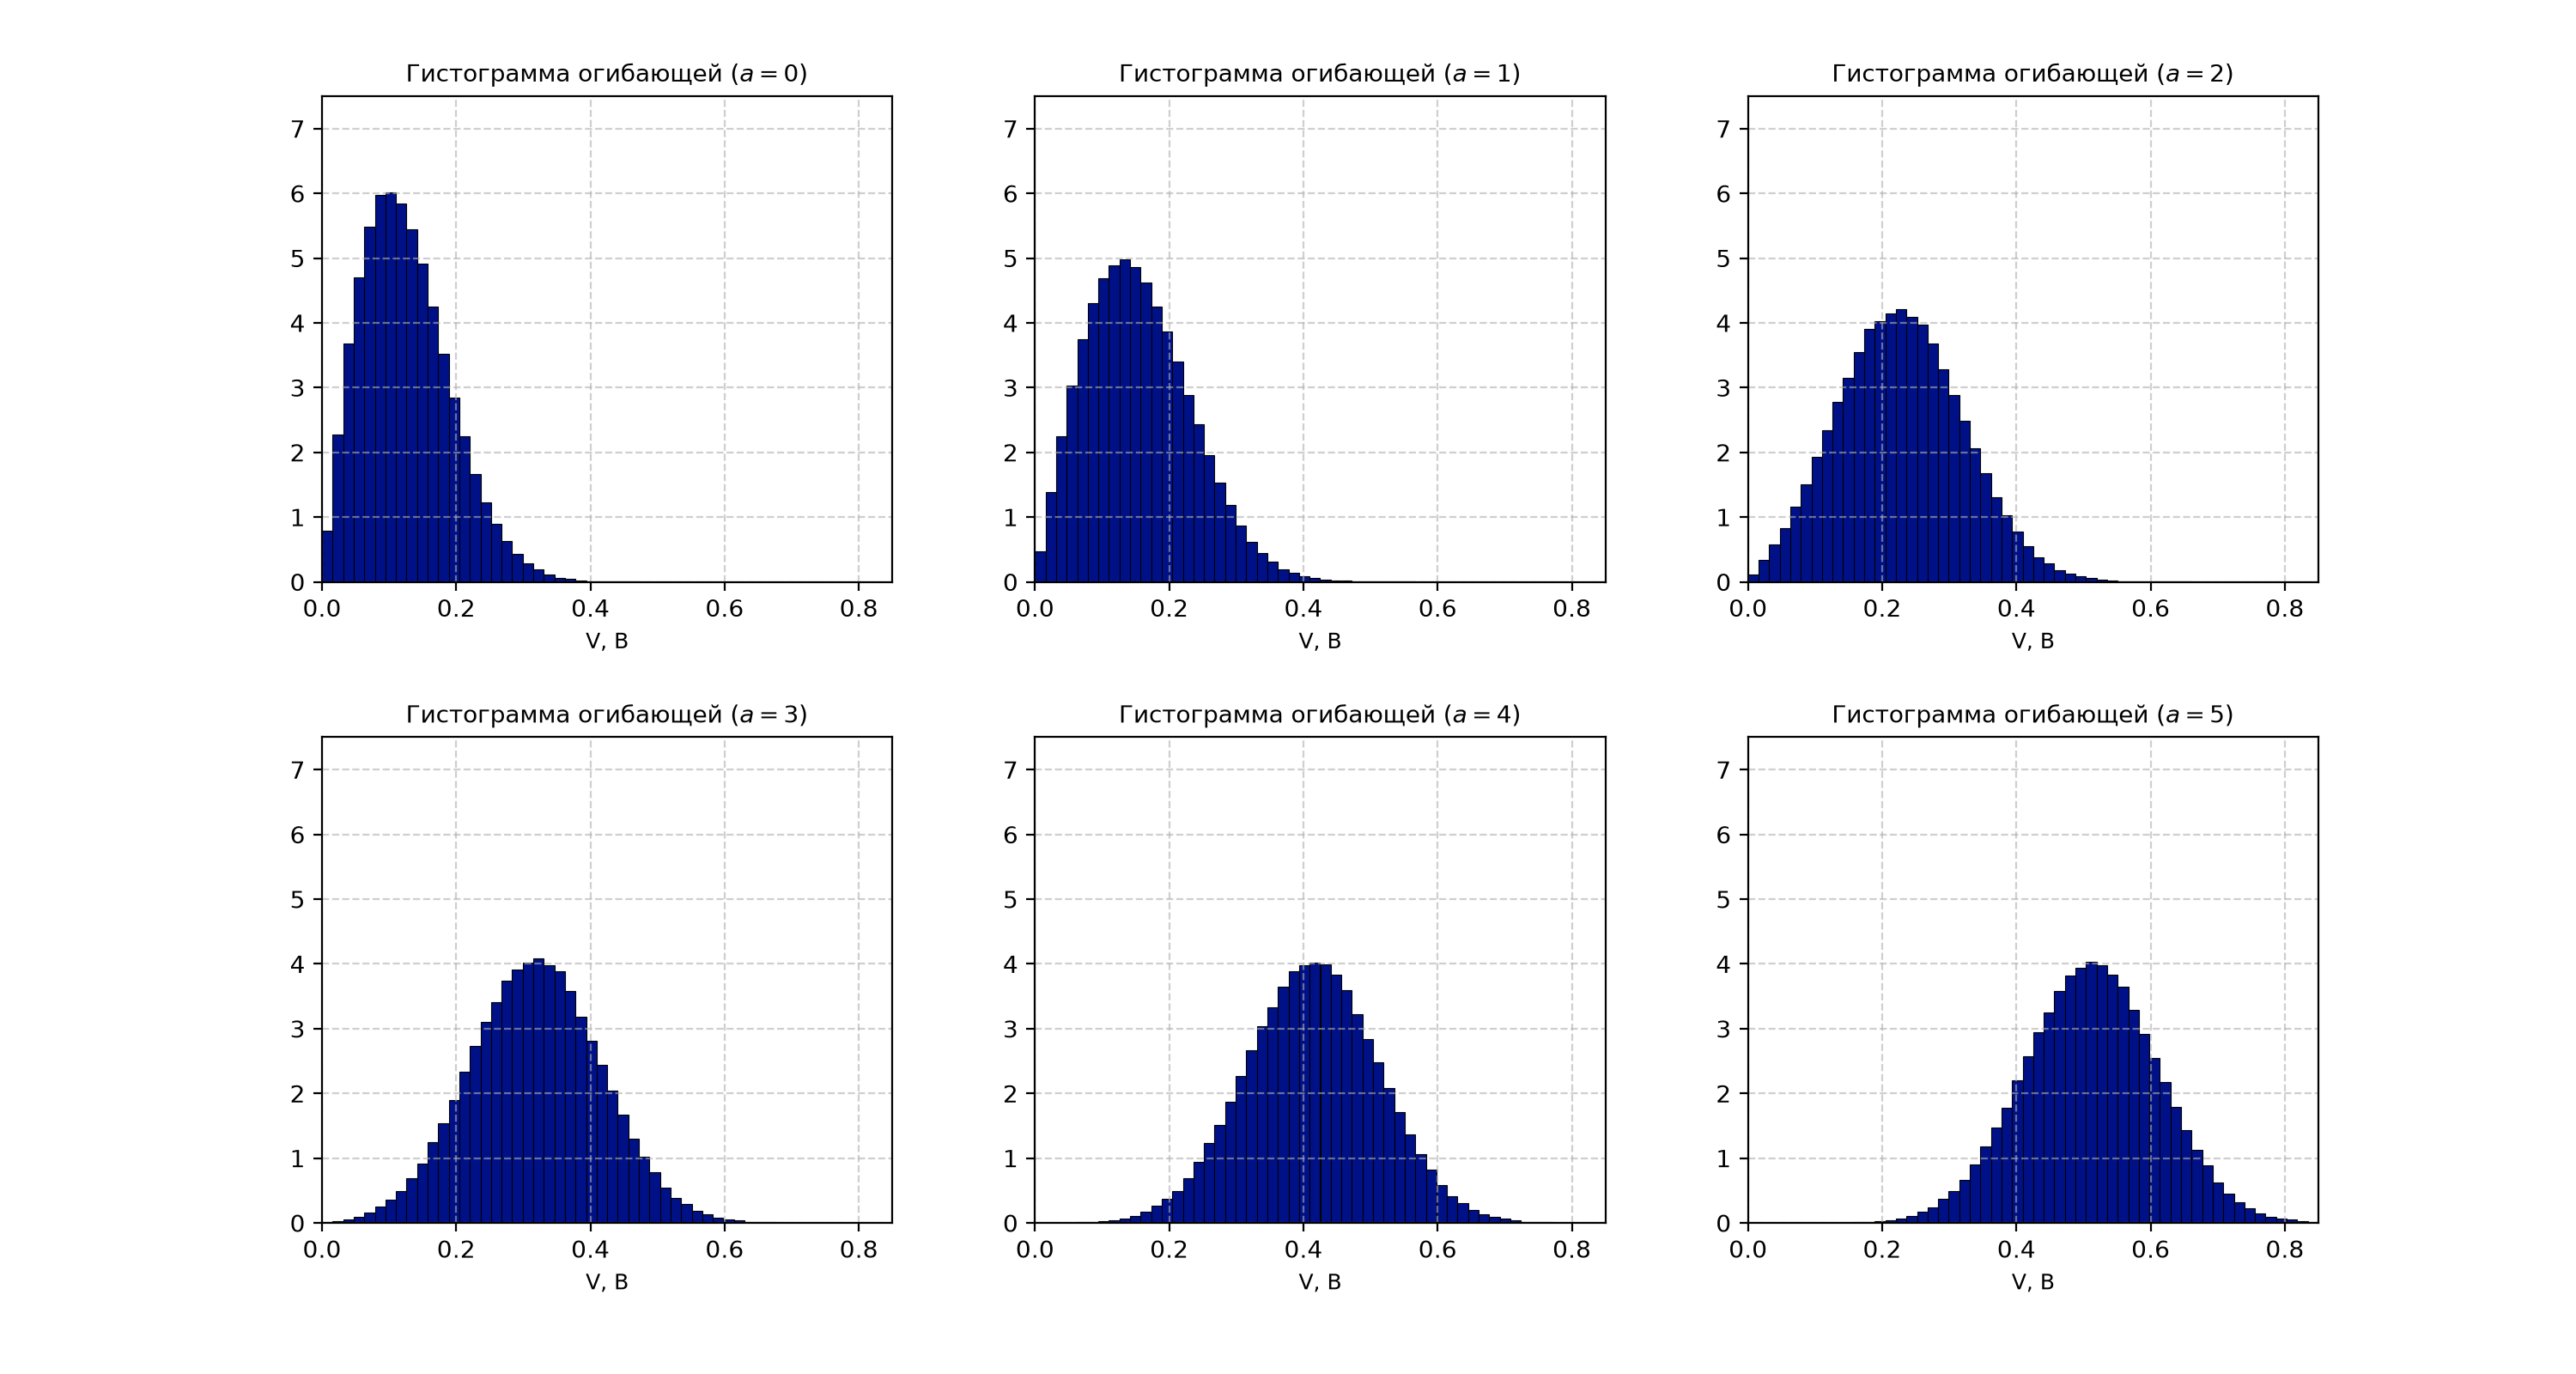
\includegraphics[width=0.96\linewidth]{exports_fig/pic_env_histograms_a0_a5.png}
    \caption{Гистограммы распределения огибающей при значениях отношения сигнал/шум $a = 0, 1, 2, 3, 4, 5$}
    \label{fig:env_histograms}
\end{figure}

При вариации отношения сигнал/шум $a = U_c / U_{\text{ш}}$ от $0$ до $5$ (Рис.~\ref{fig:env_histograms}) наблюдается плавная эволюция закона распределения.
При $a = 0$ плотность распределения имеет асимметричный вид и подчиняется закону Рэлея с модой в окрестности $U_{\text{ш}} = 0{,}1$~В.
При $a = 1$ и $a = 2$ распределение трансформируется в закон Райса со смещением максимума вправо.
При $a \ge 3$ распределение становится практически симметричным и хорошо аппроксимируется нормальным законом с математическим ожиданием $\overline{V} \approx U_c$ и дисперсией $\sigma_V^2 \approx \sigma_{\text{ш}}^2 = U_{\text{ш}}^2$.

\begin{figure}[H]
    \centering
    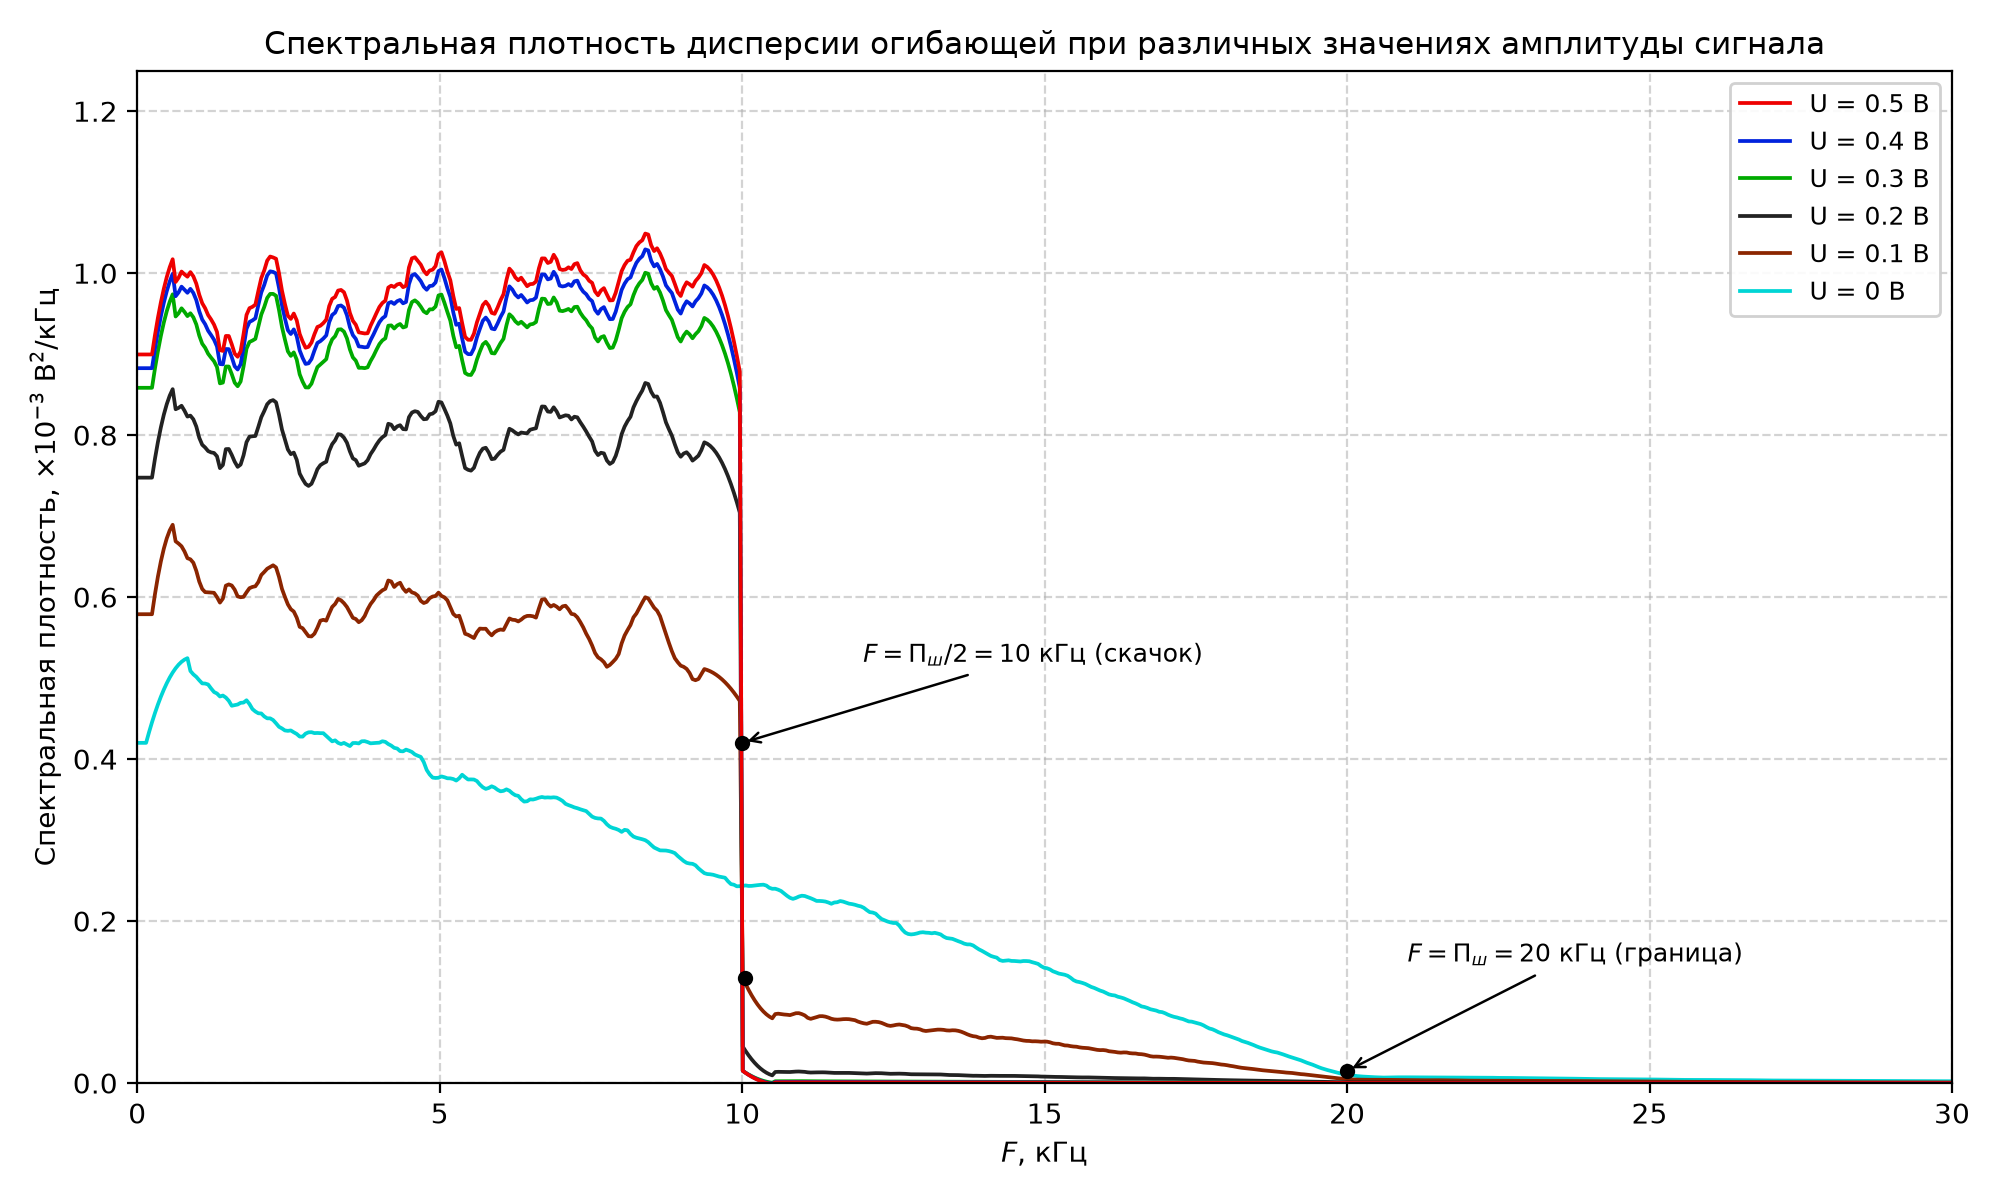
\includegraphics[width=0.85\linewidth]{exports_fig/pic_env_psd_summary.png}
    \caption{Спектральная плотность дисперсии случайной составляющей огибающей при различных амплитудах входного сигнала}
    \label{fig:env_psd_summary}
\end{figure}

Спектральная плотность дисперсии центрированной огибающей (Рис.~\ref{fig:env_psd_summary}) наглядно демонстрирует физику нелинейного взаимодействия.

В отсутствие сигнала ($U_c = 0$) спектр имеет треугольную форму с шириной $\Pi_{\text{ш}} = 20$~кГц за счет биений составляющих шума между собой.

При наличии сигнала возникают биения несущей с синфазной квадратурой шума в полосе до $\Pi_{\text{ш}}/2 = 10$~кГц, что при $U_c = 0{,}1$~В приводит к скачку уровня на частоте $10$~кГц.

При $U_c \ge 0{,}3$~В огибающая линеаризуется ($V(t) \approx U_c + U_{\text{ш}}^c(t)$), поэтому спектр принимает прямоугольную форму шириной $10$~кГц и фиксируется на предельном уровне $G(F) = 2\sigma_{\text{ш}}^2 / \Pi_{\text{ш}} = 1{,}0\cdot 10^{-3}$~В$^2$/кГц независимо от амплитуды сигнала.

\subsection{Решение задачи Д-1}
На входе блока высокочастотного усиления (БВЧ) приёмника, согласованного с антенной с шумовой температурой $T_{\text{А}} = 100$~К, действует амплитудно-модулированный (АМ) сигнал со $100\%$-й модуляцией ($m = 1{,}0$) с эффективным напряжением несущей $U_{\text{нес}} = 1{,}6$~мкВ. БВЧ имеет параметры: входное сопротивление $R_{\text{вх}} = 75$~Ом, коэффициент шума $K_{\text{ш}} = 6$~дБ ($K_{\text{ш}} \approx 3{,}98$), шумовая полоса пропускания $\Pi_{\text{ш}} = 8$~МГц, коэффициент усиления $K_{0\,\text{БВЧ}} = 10^4$.
\begin{enumerate}
    \item Изменится ли отношение сигнал-шум на выходе приемника, если заменить диодный линейный амплитудный детектор синхронным амплитудным детектором (при условии идеальной синхронизации?)
    \item Если изменится, то насколько децибел?
\end{enumerate}

\paragraph{Решение. }
Эффективная шумовая температура приёмника, приведенная к его входу:
\begin{equation}
    T_{\text{пр}} = T_0 (K_{\text{ш}} - 1) = 290 \cdot (3{,}981 - 1) \approx 864{,}5~\text{К},
\end{equation}
где $T_0 = 290$~К — стандартная температура.

Результирующая шумовая температура системы «антенна — вход БВЧ»:
\begin{equation}
    T_{\Sigma} = T_{\text{А}} + T_{\text{пр}} = 100 + 864{,}5 = 964{,}5~\text{К}.
\end{equation}

Мощность шума на входе БВЧ в согласованном тракте полосой $\Pi_{\text{ш}} = 8$~МГц:
\begin{equation}
    P_{\text{ш}} = k T_{\Sigma} \Pi_{\text{ш}} = 1{,}38 \cdot 10^{-23} \cdot 964{,}5 \cdot 8 \cdot 10^6 \approx 1{,}065 \cdot 10^{-13}~\text{Вт},
\end{equation}
где $k = 1{,}38 \cdot 10^{-23}$~Дж/К — постоянная Больцмана.

Эффективное напряжение шума на входе БВЧ:
\begin{equation}
    U_{\text{ш, вх}} = \sqrt{P_{\text{ш}} R_{\text{вх}}} = \sqrt{1{,}065 \cdot 10^{-13} \cdot 75} \approx 2{,}83~\text{мкВ}.
\end{equation}

Амплитуда немодулированной несущей входного сигнала:
\begin{equation}
    U_{c m} = \sqrt{2} \cdot U_{\text{нес}} = \sqrt{2} \cdot 1{,}6 \approx 2{,}26~\text{мкВ}.
\end{equation}

Отношение сигнал/шум по напряжению на входе детектора:
\begin{equation}
    a = \frac{U_{c m}}{U_{\text{ш, вх}}} = \frac{2{,}26}{2{,}83} \approx 0{,}80 \approx 1{,}0.
\end{equation}

При $a \approx 1$ линейный амплитудный детектор переходит в квазилинейный режим работы ($q_{\text{вых}} \approx m^2 q_{\text{вх}}$). 

В рамках инженерного приближения сильного сигнала характеристики линейного АД и синхронного детектора сближаются, поэтому отношение сигнал/шум на выходе приёмника практически неизменятся

\begin{figure}[H]
    \centering
    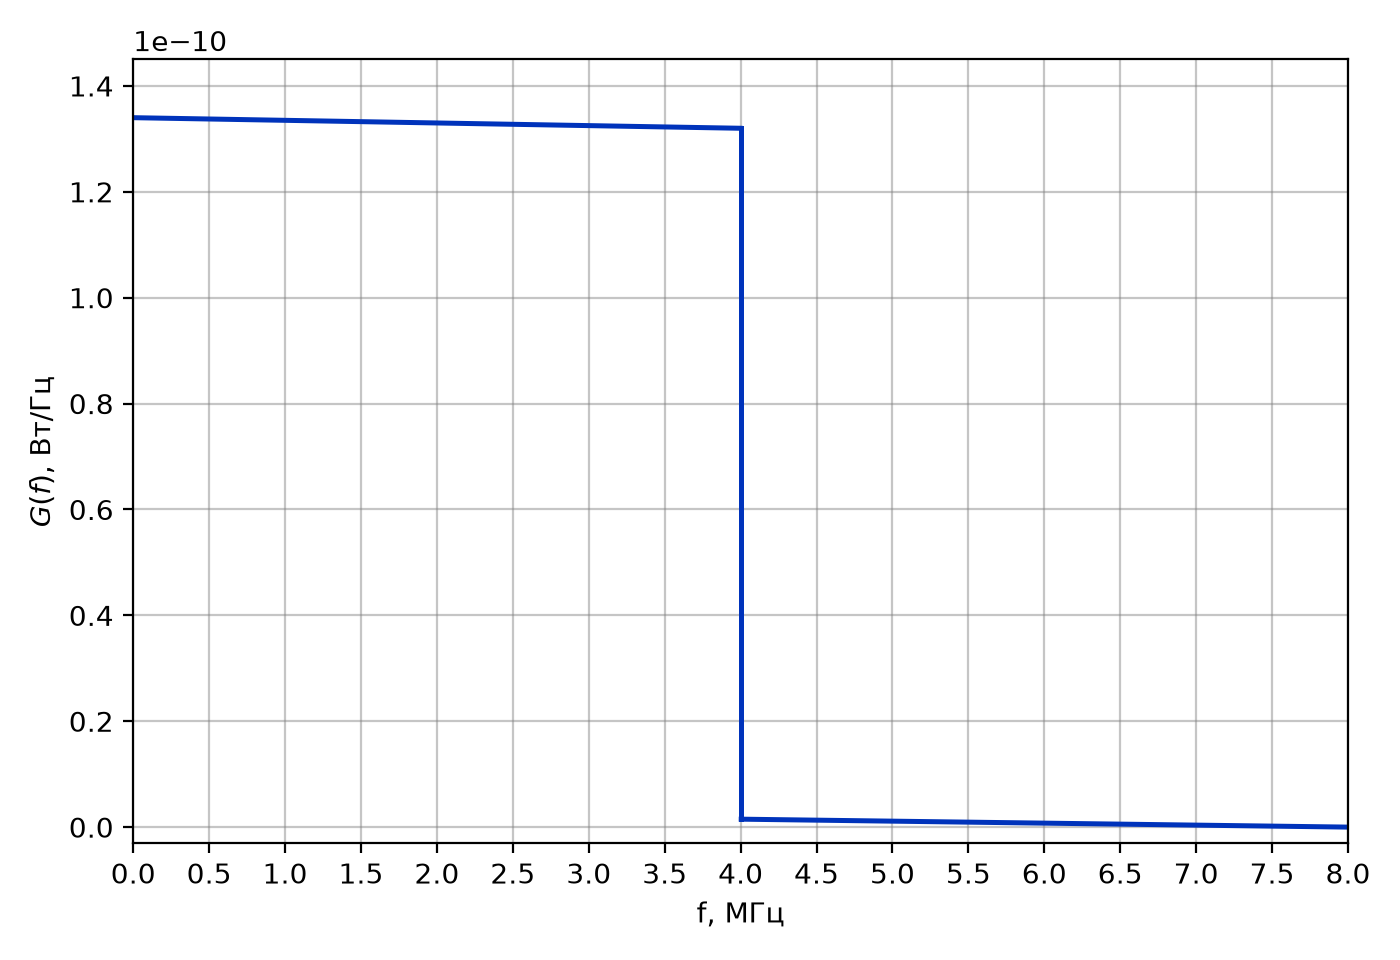
\includegraphics[width=0.75\linewidth]{exports_fig/pic_task_d1_a3.png}
    \caption{График СПШ на выходе линейного АД}
    \label{fig:task_d1_a3}
\end{figure}

\begin{figure}[H]
    \centering
    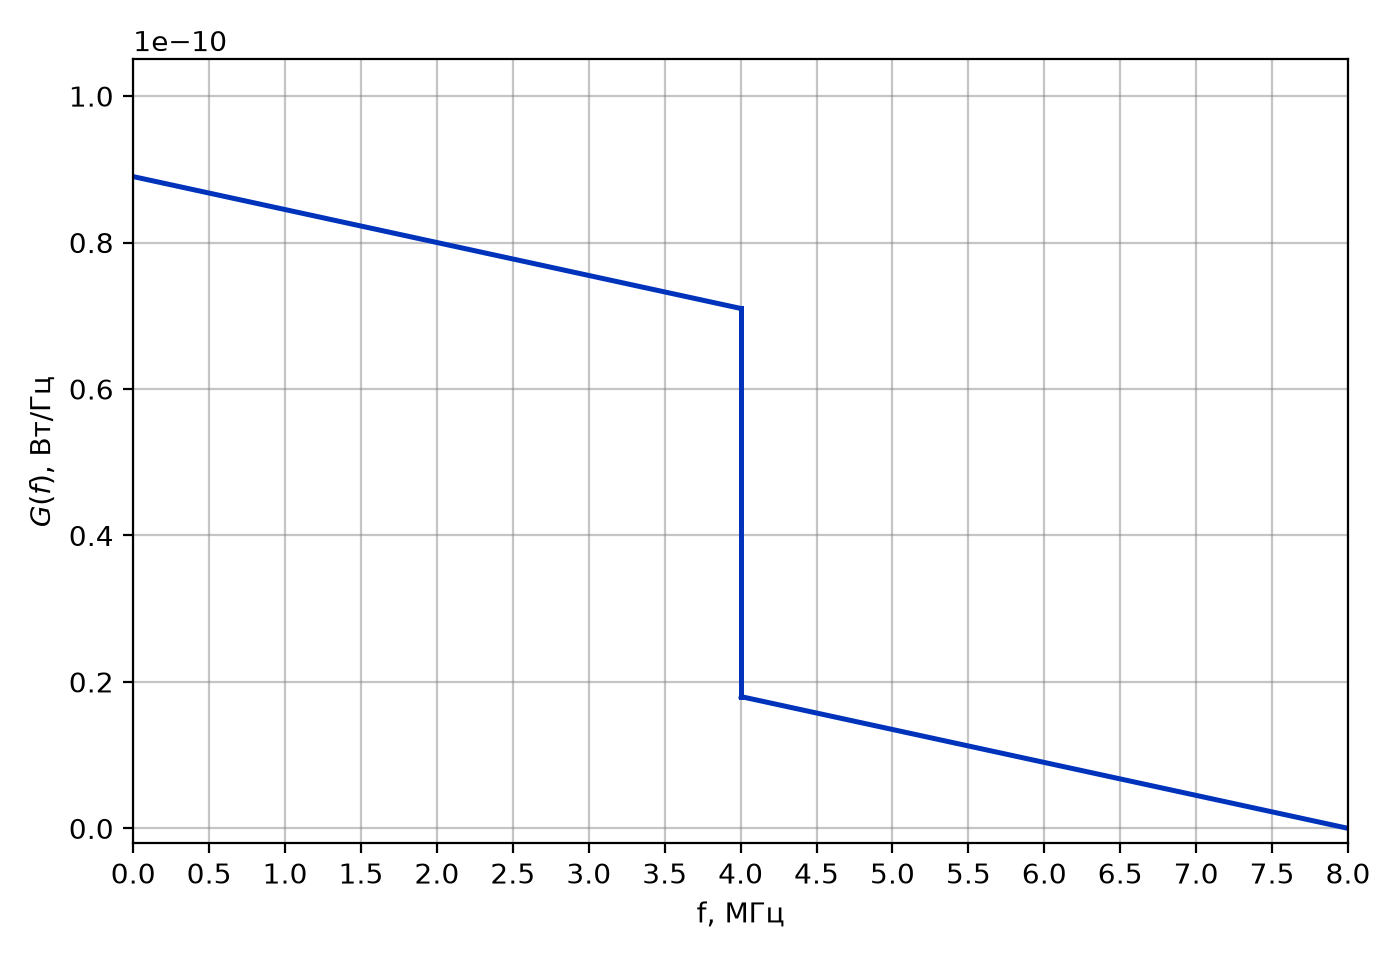
\includegraphics[width=0.75\linewidth]{exports_fig/pic_task_d1_a1.png}
    \caption{График СПШ на выходе линейного АД при $a = 1$}
    \label{fig:task_d1_a1}
\end{figure}

